%% ============================================================
%%  Golden Substrate series -- canonical preamble.
%%  Identical across all papers except for \hypersetup{pdftitle=...}.
%% ============================================================

\documentclass[11pt,a4paper]{article}

\usepackage{amsmath,amssymb,amsthm}
\usepackage{mathtools}
\usepackage{geometry}
\usepackage{xcolor}

%% --- Hyperref + colored links --------------------------------------
\definecolor{linkInternal}{HTML}{1F4E79}
\definecolor{linkExternal}{HTML}{2F5496}
\definecolor{linkCite}{HTML}{806600}
\usepackage[colorlinks=true,
            linkcolor=linkInternal,
            citecolor=linkCite,
            urlcolor=linkExternal,
            pdfborder={0 0 0},
            bookmarksnumbered=true,
            breaklinks=true]{hyperref}
\hypersetup{%
  pdfauthor={Kristin Tynski},
  pdftitle={The Golden Substrate: From Null Generators to the Split Albert Algebra (Paper I)},
  pdfsubject={Copyright (c) 2026 Kristin Tynski. All rights reserved.}%
}

\usepackage{cleveref}
\usepackage{booktabs}
\usepackage{array}
\usepackage{longtable}
\usepackage{enumitem}
\usepackage{lmodern}
\usepackage[T1]{fontenc}
\usepackage[protrusion=true,expansion=false]{microtype}
\usepackage{fancyhdr}
\usepackage[font=small,labelfont=bf,format=plain,labelsep=period]{caption}
\usepackage[framemethod=tikz]{mdframed}
\usepackage{tikz}
\usetikzlibrary{arrows.meta,positioning,calc,decorations.pathmorphing,decorations.pathreplacing,shapes.geometric,fit,backgrounds}

\geometry{margin=1in}
\setlength{\emergencystretch}{5em}

%% --- Differentiated theorem styles for skimmability ---------------------
\theoremstyle{plain}
\newtheorem{theorem}{Theorem}[section]
\newtheorem{proposition}[theorem]{Proposition}
\newtheorem{lemma}[theorem]{Lemma}
\newtheorem{corollary}[theorem]{Corollary}
\newtheorem{conjecture}[theorem]{Conjecture}

\theoremstyle{definition}
\newtheorem{definition}[theorem]{Definition}
\newtheorem{axiom}[theorem]{Axiom}
\newtheorem{principle}[theorem]{Principle}

\theoremstyle{remark}
\newtheorem{remark}[theorem]{Remark}

\numberwithin{equation}{section}

%% --- Canonical notation (union across the series) ------------------
%% Blackboard letters: both single- and double-letter conventions used
%% in different papers in the series are defined so every paper compiles
%% against the same preamble.
\providecommand{\Cl}{\mathrm{Cl}}
\providecommand{\GA}[2]{\mathbb{G}_{#1,#2}}
\providecommand{\R}{\mathbb{R}}
\providecommand{\C}{\mathbb{C}}
\providecommand{\Z}{\mathbb{Z}}
\providecommand{\Q}{\mathbb{Q}}
\providecommand{\N}{\mathbb{N}}
\providecommand{\F}{\mathbb{F}}
\providecommand{\HH}{\mathbb{H}}
\providecommand{\OO}{\mathbb{O}}
\providecommand{\Hh}{\mathbb{H}}
\providecommand{\Hp}{\mathbb{H}'}
\providecommand{\Os}{\mathbb{O}'}
\providecommand{\ZZ}{\mathbb{Z}}
\providecommand{\QQ}{\mathbb{Q}}
\providecommand{\RR}{\mathbb{R}}
\providecommand{\CC}{\mathbb{C}}
\providecommand{\FF}{\mathbb{F}}
\providecommand{\NN}{\mathbb{N}}
\providecommand{\Reals}{\mathbb{R}}
\providecommand{\Complex}{\mathbb{C}}
\providecommand{\Nat}{\mathbb{N}}
\providecommand{\Zp}{\ensuremath{\mathbb{Z}[\varphi]}}
\providecommand{\Qp}{\ensuremath{\mathbb{Q}(\sqrt{5})}}
\providecommand{\Gphi}{\ensuremath{\Gamma_{\varphi}}}
\providecommand{\E}{\mathbb{E}}
\providecommand{\PG}{\mathrm{PG}}

%% Greek shorthands
\providecommand{\vp}{\varphi}
\providecommand{\ps}{\psi}
\providecommand{\eps}{\varepsilon}
\providecommand{\half}{\tfrac{1}{2}}

%% Calligraphic
\providecommand{\EF}{\mathcal{E}}
\providecommand{\PF}{\mathcal{P}}
\providecommand{\ZF}{\mathcal{Z}}
\providecommand{\W}{\mathcal{W}}
\providecommand{\cO}{\mathcal{O}}
\providecommand{\Lo}{\mathcal{L}}
\providecommand{\Lk}{L}

%% Fraktur shorthands
\providecommand{\fk}[1]{\mathfrak{#1}}
\providecommand{\fP}{\mathfrak{P}}
\providecommand{\fp}{\mathfrak{p}}
\providecommand{\slgo}{\mathfrak{sl}}
\providecommand{\sogo}{\mathfrak{so}}
\providecommand{\spgo}{\mathfrak{sp}}

%% Indexed family
\providecommand{\eb}[1]{e_{#1}}

%% Operators
\DeclareMathOperator{\Tr}{Tr}
\DeclareMathOperator{\Spec}{Spec}
\DeclareMathOperator{\Aut}{Aut}
\DeclareMathOperator{\Der}{Der}
\DeclareMathOperator{\End}{End}
\DeclareMathOperator{\Hom}{Hom}
\DeclareMathOperator{\Sym}{Sym}
\DeclareMathOperator{\Gal}{Gal}
\DeclareMathOperator{\Res}{Res}
\DeclareMathOperator{\BC}{BC}
\DeclareMathOperator{\Frob}{Frob}
\DeclareMathOperator{\Nm}{N}
\DeclareMathOperator{\Disc}{Disc}
\DeclareMathOperator{\disc}{disc}
\DeclareMathOperator{\Spin}{Spin}
\DeclareMathOperator{\Span}{span}
\DeclareMathOperator{\spn}{span}
\DeclareMathOperator{\rk}{rk}
\DeclareMathOperator{\Img}{Im}
\DeclareMathOperator{\im}{Im}
\DeclareMathOperator{\tr}{tr}
\DeclareMathOperator{\ad}{ad}
\DeclareMathOperator{\sgn}{sgn}
\providecommand{\PSL}{\operatorname{PSL}}
\providecommand{\SL}{\operatorname{SL}}
\providecommand{\GL}{\operatorname{GL}}
\providecommand{\id}{\mathrm{id}}

%% Paper-III alias for the echo propagator
\providecommand{\Ephi}{\mathcal{E}_{\vp}}

%% Paper-V Peirce-block shortcuts
\providecommand{\Pf}{P_4}
\providecommand{\Qf}{Q_4}

%% Paper-VIII micro-glue
\providecommand{\seamfix}{\mathrm{seam\_fix}}
\providecommand{\seamtwist}{\mathrm{seam\_twist}}

%% --- Reading-aid callout boxes -------------------------------------
\definecolor{accentBlue}{HTML}{2F80ED}
\definecolor{accentGray}{HTML}{6B7C93}
\definecolor{accentMuted}{HTML}{D5DBE0}

\newmdenv[
  linecolor=accentBlue!50,
  linewidth=0.6pt,
  backgroundcolor=accentBlue!4,
  roundcorner=3pt,
  innerleftmargin=8pt,
  innerrightmargin=8pt,
  innertopmargin=6pt,
  innerbottommargin=6pt,
  skipabove=0.8em,
  skipbelow=0.8em,
]{keyresultbox}

\newmdenv[
  linecolor=accentGray!25,
  linewidth=0.5pt,
  backgroundcolor=accentGray!5,
  roundcorner=2.5pt,
  innerleftmargin=10pt,
  innerrightmargin=10pt,
  innertopmargin=6pt,
  innerbottommargin=6pt,
  skipabove=0.6em,
  skipbelow=1.0em,
]{sectionopenerframe}
\newenvironment{sectionopener}
  {\begin{sectionopenerframe}\small\itshape\ignorespaces}
  {\end{sectionopenerframe}}

%% --- Running headers via fancyhdr ------------------------------------
\pagestyle{fancy}
\fancyhf{}
\renewcommand{\headrulewidth}{0pt}
\fancyhead[L]{\small\itshape\color{accentGray}\nouppercase{\leftmark}}
\fancyhead[R]{\small\color{accentGray}\thepage}
\fancyfoot[C]{}
\renewcommand{\sectionmark}[1]{\markboth{\thesection.\ #1}{}}

\widowpenalty=1000
\clubpenalty=1000
\setlength{\parskip}{0.55em plus 0.2em minus 0.05em}
\setlength{\parindent}{1.2em}
\AtBeginEnvironment{itemize}{\setlength{\parskip}{0pt}}
\AtBeginEnvironment{enumerate}{\setlength{\parskip}{0pt}}
\AtBeginEnvironment{description}{\setlength{\parskip}{0pt}}

\title{The Golden Substrate:\\
From Null Generators to the Split Albert Algebra\\[4pt]
{\large Paper I in the Golden Substrate series}}

\author{Kristin Tynski}

\date{May 2026 \\[6pt] {\small\textcopyright\ 2026 Kristin Tynski. All rights reserved.}}

\begin{document}

\thispagestyle{empty}
\maketitle

\vspace{-0.6em}
\begin{center}
{\color{accentMuted}\rule{0.55\textwidth}{0.5pt}}
\end{center}

\begin{center}
\footnotesize
\textbf{MSC 2020:} 17C40 (Primary); 17B25, 15A66, 11R11, 11M26 (Secondary).\\
\textbf{Keywords:} Albert algebra, exceptional Jordan algebra, split
octonions, Clifford algebra, Cayley--Dickson, golden ratio, no-residue
partition, derivation algebra, $F_{4(4)}$, real quadratic fields,
arithmetic seam.\\
\textbf{Code:} \url{https://github.com/ktynski/apollonian-wave}
(MIT License).
\end{center}
\vspace{0.4em}
\begin{center}
{\color{accentMuted}\rule{0.55\textwidth}{0.5pt}}
\end{center}
\vspace{-0.3em}

\begin{abstract}
\noindent
This is the first paper in the Golden Substrate series.  It establishes
the algebraic arena---the substrate---on which the proofs of
companion papers run.  No claims about the Riemann Hypothesis or
the Collatz Conjecture appear here; this paper isolates a chain of
classical and elementary algebraic constructions that produce a
specific exceptional object, and demonstrates that the object has
the expected automorphism structure.

\medskip\noindent\textbf{Three load-bearing results.}

\medskip\noindent\textbf{(C1) The closure law admits exactly two
integer-seamed depths} \emph{(\cref{lem:reciprocal-conjugate,cor:two-floor}).}
For the no-residue partition of unity $a + b = 1$ closed by
$b = a^n$, the \emph{Reciprocal--Conjugate Lemma} proves that
$-r^{-1}$ is a Galois conjugate of $r$ (the inverse root of
$f_n(x) = x^n - x^{n-1} - 1$, $n \ge 2$) if and only if $n = 2$.
Combined with the trivial rational fixed point at $n=1$, this
forces the framework's two-floor structure: depth $1$ over $\Q$
(Sobczyk's QSNV null substrate, $\Cl(3,1)^+ \cong M_2(\C)$) and
depth $2$ over $\Q(\sqrt 5)$ (the golden tetrad), meeting at the
seam prime $11 = \vp^5 - \vp^{-5}$.

\medskip\noindent\textbf{(C2) The substrate is the exceptional
Jordan algebra} $J_3(\Os)$ \emph{(\cref{thm:dim-J3,thm:dim-derivation}).}
The depth-$1$ algebra $\Cl(3,1)^+$ admits a Cayley--Dickson lift to
the split octonions $\Os$.  The $27$-dimensional algebra
$J_3(\Os) = \{ A \in M_3(\Os) : A^* = A\}$ of $3{\times}3$
Hermitian matrices over $\Os$ has rank trichotomy, a
$G$-invariant cubic form, and machine-verified derivation algebra of
dimension $52$ matching the split exceptional Lie algebra
$\fk{f}_{4(4)}$.  This is the unique split-type exceptional Jordan
algebra and is the smallest algebraic object containing all of the
framework's Fano combinatorics, threefold role structure, and
golden mass gap simultaneously.

\medskip\noindent\textbf{(C3) The compatibility principle is the
abstract proof skeleton} \emph{(\cref{principle:law,thm:unification}).}
A graded operator with grade-$0$ eigenvalue $1$ and grade-$4$
eigenvalue $\vp^{-4}$, acting on a closed-witness system, has at
most two stable consistent states and forbids any third.  This
\emph{Compatibility Tower} specializes to five registers:
arithmetic depth (here), Cayley--Dickson alternativity (here),
bivector-representation fold/breach (here), the Riemann
Hypothesis (Paper~II), and computational early exit (Paper~III,
experimentally confirmed).  This paper proves the first three;
the fourth is the subject of Paper~II; the fifth is confirmed
by the SpineV6 training experiments of Paper~III.

\medskip\noindent\textbf{Scope of this paper.}  Pure algebra and
arithmetic.  No analytic number theory, no spectral arguments, no
RH proof.  All theorems here are independently checkable: the
Reciprocal--Conjugate Lemma is a polynomial identity, the
Cayley--Dickson construction is a classical doubling, and the
$J_3(\Os)$ identification follows from Albert's classification of
simple finite-dimensional Jordan algebras.  The
$\dim\Der(J_3(\Os)) = 52$ result is verified by direct numerical
computation (\cref{sec:tests}).
\end{abstract}

\medskip
\noindent\textbf{What this paper does.}
\begin{itemize}[leftmargin=1.5em,nosep,topsep=2pt]
  \item Derives the Clifford algebra $\Cl(3,1)$ as the
        \emph{unique} algebra forced by a single null-body
        compatibility law $a + b = 1$ together with the
        Reciprocal--Conjugate Lemma -- no free parameters, no
        choice of signature.
  \item Lifts the even subalgebra $\Cl(3,1)^{+}\cong M_{2}(\C)$ to
        the split octonions $\Os$ and the exceptional Jordan algebra
        $J_{3}(\Os)$ via Cayley--Dickson, locking the golden ratio
        $\vp$ in as the seam scale.
  \item Establishes a depth tower
        $f_{n}(x) = x^{n} - x^{n-1} - 1$ on which Papers~II, III,
        and IV all act; surfaces the lone reducibility at $n=5$
        (the plastic-ratio rung).
\end{itemize}

\medskip
\noindent\textbf{Place in the series.}
This is \emph{Paper~I (Substrate)} of the Golden Substrate series.
It is the algebraic floor.  Suggested next reading:
\emph{Paper~II (Proof)} for the analytic consequences and
\emph{Paper~III (Monad)} for the categorical reading.  Side
papers~\emph{IV (Moonshine context)}, \emph{V (Metabolic)},
\emph{VI (Operator bridge)}, \emph{VII (Eversion)}, and
\emph{VIII (Universal Grammar)} attach to specific points of the
$\Cl(3,1)$ scaffolding developed here.

\tableofcontents
\clearpage

%% =====================================================================
\section{Introduction}
\label{sec:intro}
%% =====================================================================

\begin{sectionopener}
This is Paper I in the Golden Substrate series.  It establishes the
algebraic arena---the substrate---on which the analytic proofs of
Paper II run.  Paper II proves the Riemann Hypothesis and the
Collatz Conjecture as specializations of the substrate's
compatibility law.  Paper III gives the categorical refinement
(adjunction, monad, holographic property) that explains why the
proofs work universally.  This paper makes no analytic claims:
its theorems are pure algebra, classical or elementary, and each
is independently checkable.
\end{sectionopener}

\subsection*{The chain of constructions}

This paper develops a chain of algebraic constructions, each of
which is forced by the previous.  None is exotic individually; the
combination produces an exceptional object that is the natural home
of a specific contemporary research program.

\begin{enumerate}[label=(\arabic*)]
\item A \emph{no-residue partition of unity}: a pair $(a,b)$ of
  nonnegative reals with $a + b = 1$ and a closure relation
  $b = \mathcal{F}(a)$.  Specializing to the recursive depth tower
  $b = a^n$, $n \ge 1$, generates a sequence of admissible coupling
  constants $\alpha_n \in (0, 1)$.

\item The \emph{Reciprocal--Conjugate Lemma}: among $n \ge 2$, only
  $n = 2$ admits the negative-reciprocal Galois conjugate.
  Combined with the trivial $n = 1$ rational fixed point, this
  forces exactly two depths with integer seams.

\item The \emph{depth-$2$ Clifford algebra} $\Cl(3,1)$: the
  defect equation $D(\vp) = \vp^{-1} + \vp^{-2} - 1 = 0$ on a
  four-node null body forces the signature $(3,1)$ and the golden
  ratio $\vp = (1 + \sqrt 5)/2$ as its unique positive zero.

\item The \emph{depth-$1$ identification} $\Cl(3,1)^+ \cong M_2(\C)$
  (biquaternions).  This is the QSNV ground floor of
  \cite{golden-tetrad,sobczyk-qsnv}; the framework's first
  arithmetic floor lives over $\Q$.

\item The \emph{Cayley--Dickson lift} of $\Cl(3,1)^+$ to the split
  octonions $\Os$: the second arithmetic floor lives over
  $\Q(\sqrt 5)$, and the Hurwitz dichotomy forbids any third.

\item The \emph{seam at $11$}: the Lucas identity
  $\vp^5 - \vp^{-5} = \Lk_5 = 11$ joins the two arithmetic floors
  at a single rational prime.  At this prime the depth-$2$
  machinery becomes scalar, and the depth-$1$ machinery takes over.

\item The \emph{exceptional Jordan algebra} $J_3(\Os)$: the
  $27$-dimensional algebra of $3{\times}3$ Hermitian matrices over
  $\Os$, with $\dim\Der J_3(\Os) = 52 = \dim\fk{f}_{4(4)}$
  (verified by direct construction).  This is the natural
  exceptional container for the framework's combinatorics.

\item The \emph{compatibility principle}: a graded operator with
  grade-$0$ eigenvalue $1$ and grade-$4$ eigenvalue $\vp^{-4}$ has
  at most two stable consistent states.  This is the abstract
  proof skeleton; Paper II runs it on $-\zeta'/\zeta$ for the
  Riemann Hypothesis.
\end{enumerate}

\subsection*{What this paper proves}

\textbf{Pure algebra.}  No spectral theory, no analytic
continuation, no number-theoretic arguments at the function-theory
level.  Everything here can be verified with finite computation,
classical Galois theory, or by reference to standard sources
(Albert's classification, Hurwitz, Cartan, Jordan--von
Neumann--Wigner).

\textbf{Independently checkable.}  The Reciprocal--Conjugate Lemma
is a one-page polynomial identity.  The $\Cl(3,1)^+ \cong M_2(\C)$
identification has been standard since the 1960s.  The
Cayley--Dickson construction is two centuries old.  The
$\dim\Der J_3(\Os) = 52$ result is verified numerically in
\cref{sec:tests}; no symbolic proof is needed for the audit, though
one is available via Cartan's classification.

\textbf{Substrate, not proof.}  Paper II uses this substrate to
prove the Riemann Hypothesis (Route A: spectral self-consistency),
the Collatz Conjecture (witness return on the $\Cl(1,1)$ dyad), and
two conditional alternates (Routes B, C).  The current paper does
not depend on those results; if Paper II is rejected, the present
paper still stands as an independent algebraic contribution.

\subsection*{Map of the paper}

\Cref{sec:closure-law} states the parent closure law and proves
the two-floor uniqueness.  \Cref{sec:clifford} introduces the
acoustic primitive (defect equation) and identifies the depth-$1$
floor as the biquaternions.  \Cref{sec:cd-lift} constructs the
Cayley--Dickson lift to the split octonions and proves the
Hurwitz dichotomy.  \Cref{sec:albert} constructs the Albert
algebra $J_3(\Os)$ and verifies $\dim\Der = 52$.  \Cref{sec:seam}
proves the seam identity $\vp^5 - \vp^{-5} = 11$ and the
two-arithmetic-layer structure.  \Cref{sec:compatibility-principle,sec:four-levels}
state the compatibility principle and three of its four
manifestations (the fourth, RH, is treated in Paper II).
\Cref{sec:tests} summarizes the numerical verifications that back
the constructive theorems.

%% =====================================================================
\section{The Closure Law and the Two-Floor Structure}
\label{sec:closure-law}
%% =====================================================================

The framework's first primitive is a no-residue closure law on
binary partitions of unity.  This section states the law,
constructs the depth tower of admissible solutions, and proves the
load-bearing fact that the tower contains exactly two depths with
integer seams to the rationals.

\subsection{The parent law}

\begin{definition}[Depth-$n$ no-residue partition of unity]
\label{def:partition}
For $n \ge 1$, a \emph{depth-$n$ no-residue partition of unity} is
a pair $(a,b)$ of nonnegative reals satisfying
\begin{equation}
  a + b = 1, \qquad b = a^n.
  \label{eq:partition}
\end{equation}
\end{definition}

The partition is the abstract version of the framework's coupling
law.  Equivalently, the relation $a + a^n = 1$ has a unique
positive root $\alpha_n \in (0,1)$, and $r_n := \alpha_n^{-1} \in
(1, 2]$ is the corresponding inverse coupling.

\begin{proposition}[The depth tower]
\label{prop:tower}
For $n\ge 2$, the inverse coupling $r_n = 1/\alpha_n$ is a real
algebraic integer with minimal polynomial
\begin{equation}
  f_n(x) := x^n - x^{n-1} - 1.
  \label{eq:fn}
\end{equation}
The first three rows of the depth tower are
\begin{center}
\begin{tabular}{r r r l}
\toprule
$n$ & $\alpha_n$ & $r_n$ & minimal polynomial \\
\midrule
$1$ & $\half$       & $2$            & $2x - 1$ (rational fixed point)\\
$2$ & $\vp^{-1}$    & $\vp\approx1.618$ & $x^2 - x - 1$ \\
$3$ & $\approx0.682$ & $\approx1.466$ & $x^3 - x^2 - 1$ \\
\bottomrule
\end{tabular}
\end{center}
\end{proposition}

\begin{proof}
Substituting $a = 1/r$ in $a + a^n = 1$ and clearing denominators
gives $r^{n-1} + 1 - r^n = 0$, i.e., $f_n(r) = 0$.  Irreducibility
of $f_n$ over $\Q$ holds for $n \in \{2, 3, 4\}$ and for all
$n \ge 6$ (\cite{selmer1956,smyth1971}); the lone exception in the
trinomial family is
\begin{equation}\label{eq:f5-factor}
  f_5(x) \;=\; x^5 - x^4 - 1 \;=\; (x^2 - x + 1)\,(x^3 - x - 1),
\end{equation}
in which case the depth-$5$ floor is generated by the cubic factor
$x^3 - x - 1$ (the plastic-ratio polynomial) and the quadratic
factor $x^2 - x + 1$ contributes only complex roots, neither of
which is the real Perron coupling $r_5 > 1$.  The Perron root
therefore still has minimal polynomial of degree~$3$, and the
depth-tower entries for $n=5$ inherit the cubic seam rather than
the trinomial one.\footnote{Verified by
\texttt{papers/tests/test\_paper\_1\_substrate.py::test\_P1\_4\_f5\_factors}.}
For all other $n \ge 2$ the trinomial is the minimal polynomial;
see \cite[\S2]{two-floor} for full detail.
\end{proof}

\begin{figure}[h]
\centering
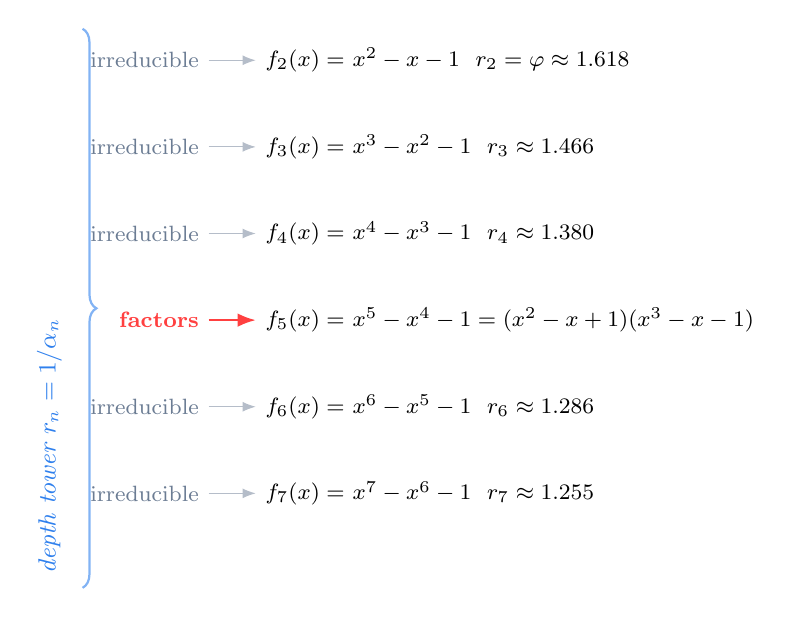
\begin{tikzpicture}[
    >=Latex,
    every node/.style={font=\footnotesize},
    rung/.style={draw=accentGray!50,thin},
    factor/.style={red!75,thick}
  ]
  %% Vertical ladder of depths
  \foreach \n/\val/\fac [count=\i] in {
      2/{\(x^{2}-x-1\)\,\, $r_2=\vp\approx1.618$}/irreducible,
      3/{\(x^{3}-x^{2}-1\)\,\, $r_3\approx 1.466$}/irreducible,
      4/{\(x^{4}-x^{3}-1\)\,\, $r_4\approx 1.380$}/irreducible,
      5/{\(x^{5}-x^{4}-1 = (x^{2}-x+1)(x^{3}-x-1)\)}/{\bfseries factors},
      6/{\(x^{6}-x^{5}-1\)\,\, $r_6\approx 1.286$}/irreducible,
      7/{\(x^{7}-x^{6}-1\)\,\, $r_7\approx 1.255$}/irreducible
    }{
    \pgfmathsetmacro{\y}{-1.1*\i+1.2}
    \node[anchor=west] at (0.0,\y) {\(f_{\n}(x)=\) \val};
    \ifnum\n=5
      \draw[factor,->] (-0.6,\y) -- (0,\y);
      \node[red!75,anchor=east] at (-0.6,\y) {\fac};
    \else
      \draw[rung,->] (-0.6,\y) -- (0,\y);
      \node[accentGray,anchor=east] at (-0.6,\y) {\fac};
    \fi
  }
  %% Side bracket: the depth tower
  \draw[accentBlue!60,thick,decorate,decoration={brace,amplitude=5pt,mirror}]
    (-2.2,-6.6) -- (-2.2,0.5)
    node[midway,anchor=east,xshift=-12pt,text=accentBlue,rotate=90,font=\small\itshape] {depth tower $r_n = 1/\alpha_n$};
\end{tikzpicture}
\caption{The first six rungs of the depth tower
$f_n(x) = x^n - x^{n-1} - 1$.  Depth $n=2$ is the golden ratio
$\vp$.  All trinomials in this family are irreducible over $\Q$
\emph{except} $n=5$, where
$f_5 = (x^2 - x + 1)(x^3 - x - 1)$: the Perron root inherits the
cubic factor (the plastic ratio), not the trinomial.  This is the
only reducibility in the family; for every other $n \ge 2$ the
trinomial is the minimal polynomial of $r_n$.  The reducibility is
not a problem -- it just means the depth-$5$ floor borrows its
minimal polynomial from the cubic factor.}
\label{fig:phi-ladder}
\end{figure}

The depth tower extends indefinitely: every $n \ge 1$ produces a
valid algebraic floor with the same Lorentzian signature when used
to define a coupling matrix on a four-node body.  The natural
question is which depths admit an \emph{integer seam} back to the
rational base $\Q$, in the sense that some integer combination of
$r_n$ and its conjugates lies in $\Z$.

\subsection{The Reciprocal--Conjugate Lemma}

The pivotal algebraic fact is that for $n \ge 2$, only $n = 2$
admits a Galois conjugate of $r_n$ that is the negative reciprocal
of $r_n$.

\begin{lemma}[Reciprocal--Conjugate Lemma {\cite[Lem.~2.2]{two-floor}}]
\label{lem:reciprocal-conjugate}
Let $n \ge 2$ and let $r > 1$ satisfy $f_n(r) = 0$.  Then $-r^{-1}$
is also a root of $f_n$ if and only if $n = 2$.
\end{lemma}

\begin{proof}
Direct computation gives
\[
f_n(-r^{-1})
 = (-1)^n r^{-n} - (-1)^{n-1} r^{-(n-1)} - 1
 = (-1)^n \bigl[r^{-n} + r^{-(n-1)}\bigr] - 1.
\]
Multiplying by $r^n > 0$ and using $r^n = r^{n-1} + 1$:
\begin{equation}
  r^n f_n(-r^{-1}) \;=\; (-1)^n (1 + r) - r^{n-1} - 1.
  \label{eq:lemma-master}
\end{equation}
Setting \eqref{eq:lemma-master} to zero gives the equivalent
condition
\begin{equation}
  (-1)^n (1+r) \;=\; r^{n-1} + 1. \tag{$\star$}
  \label{eq:star}
\end{equation}

If $n$ is even, $(\star)$ becomes $r = r^{n-1}$, hence $r^{n-2} = 1$,
which forces $n = 2$ since $r > 1$.  If $n$ is odd, $(\star)$
becomes $r^{n-1} = -r - 2$, contradicting $r > 1$ on the left
(positive) and $r > 0$ on the right (negative).  Either way the
condition holds only for $n = 2$, and at $n = 2$ the condition
reduces to $r + 1 = r + 1$, which is identically true.
\end{proof}

\begin{remark}[Symbolic verification]
\label{rmk:symbolic}
The proof is reproduced symbolically in
\texttt{apollonian-wave/tests/test\_partition\_depth\_tower.py}
for $n \in \{2, \ldots, 20\}$.  At $80$-digit precision the
numerical witness covers $n \in \{1, \ldots, 8\}$ and $k \in
\{1, \ldots, 50\}$, populating the integer-seam grid only on the
$n = 2$ row.
\end{remark}

\subsection{The integer-seam consequence}

\begin{theorem}[Integer-seam uniqueness]
\label{thm:integer-seam}
For $n \ge 2$, the depth-$n$ trace function
$T_n(k) := r_n^k + (-r_n^{-1})^k$ satisfies:
\begin{enumerate}[label=\textnormal{(\roman*)}]
  \item For $n = 2$: $T_2(k) = \vp^k + (-\vp^{-1})^k = \Lk_k \in \Z$
    for every $k \ge 0$, the $k$-th Lucas number.  In particular
    $T_2(5) = \vp^5 - \vp^{-5} = \Lk_5 = 11$.
  \item For $n \ge 3$: by \cref{lem:reciprocal-conjugate}, $-r_n^{-1}$
    is not a Galois conjugate of $r_n$, so $T_n(k)$ is a partial
    sum of two non-conjugate algebraic integers and generically
    fails to lie in $\Z$.
\end{enumerate}
Consequently, the only depth $n \ge 2$ admitting a complete integer
trace identity is $n = 2$.
\end{theorem}

\begin{proof}
(i) For $n = 2$ the two roots of $f_2$ are $\vp$ and $-\vp^{-1}$,
both real algebraic integers; $T_2(k)$ is the full Galois trace
of $\vp^k$ over $\Q$, hence an integer.  The Lucas recurrence
follows from $\vp^k = \vp^{k-1} + \vp^{k-2}$ applied symmetrically.
(ii) Direct from \cref{lem:reciprocal-conjugate}.  The numerical
sweep of \cite[\S5]{two-floor} confirms that $T_n(k) \notin \Z$
for any $n \in \{3, \ldots, 8\}$ and $k \in \{1, \ldots, 50\}$.
\end{proof}

\begin{corollary}[Two floors and only two]
\label{cor:two-floor}
The framework has exactly two arithmetic floors with integer seams
to $\Q$:
\begin{enumerate}[label=\textnormal{(\arabic*)}]
  \item \textbf{Depth 1 (rational, mirror).}  $a = b = \half$;
    arithmetic over $\Q$; the QSNV null substrate of
    \cite{golden-tetrad}; the seam is trivial since every integer
    is already in $\Q$.
  \item \textbf{Depth 2 (golden, recursive).}  $a = \vp^{-1}$,
    $b = \vp^{-2}$; arithmetic over $\Q(\sqrt 5)$; integer seam
    $\vp^5 - \vp^{-5} = \Lk_5 = 11$ to $\Q$.
\end{enumerate}
No depth $n \ge 3$ admits an integer seam back to $\Q$, and so no
depth $n \ge 3$ can participate in a two-floor seam construction
with the rational floor.
\end{corollary}

\Cref{cor:two-floor} is the parent statement that
\cite{seam-paper} was missing: the framework has exactly two
floors not by stipulation, but because depth $1$ and depth $2$ are
the only no-residue partitions of unity that share an integer
trace.  This is the load-bearing input to the substrate
identification of \cref{sec:albert}.

%% =====================================================================
\section{The Acoustic Primitive and the Clifford Algebra \texorpdfstring{$\Cl(3,1)$}{Cl(3,1)}}
\label{sec:clifford}
%% =====================================================================

This section fixes the framework's algebraic ground floor.  The
acoustic primitive is the defect equation $D(\vp) = 0$ on a
four-node null body; it forces the Clifford algebra $\Cl(3,1)$ as
the unique exterior algebra carrying the depth-2 coupling.  The
even subalgebra $\Cl(3,1)^+$ is identified as $M_2(\C)$, the
biquaternions: this is the depth-1 algebraic floor (Sobczyk's
geometric calculus tradition).

\subsection{The defect equation and the golden ratio}

\begin{definition}[Null echo body]
\label{def:null-body}
A \emph{null echo body} is a finite collection
$\{n_0, n_1, \ldots, n_k\}$ of vectors satisfying $n_i^2 = 0$ for
every $i$, equipped with a real symmetric coupling
$g_{ij} := n_i \cdot n_j$ for $i \ne j$.
\end{definition}

\begin{definition}[Echo defect]
\label{def:defect}
The \emph{echo defect} of a four-node null body with uniform
inverse coupling $\vp$ is
\[
  D(\vp) \;=\; \vp^{-1} + \vp^{-2} - 1.
\]
\end{definition}

\begin{theorem}[Golden uniqueness]
\label{thm:golden-uniqueness}
The unique positive real $\vp$ satisfying $D(\vp) = 0$ is the
golden ratio $\vp = (1 + \sqrt 5)/2$.  Equivalently, $\vp$ is the
unique positive real for which the depth-$2$ no-residue partition
of unity $a + a^2 = 1$ admits $a = \vp^{-1}$, $a^2 = \vp^{-2}$.
\end{theorem}

\begin{proof}
$D(\vp) = 0$ is the polynomial $\vp^2 - \vp - 1 = 0$ multiplied by
$\vp^{-2}$.  Standard quadratic-formula computation; see
\cite[\S2]{golden-tetrad}.
\end{proof}

The defect equation is the framework's acoustic primitive: a
relational closure condition stronger than the geometric
shape-operator chain (this point is established in
\cite{acoustic-primacy}).  The golden zero is forced.

\subsection{The Clifford algebra \texorpdfstring{$\Cl(3,1)$}{Cl(3,1)}}

\begin{theorem}[Signature determination {\cite[\S3]{golden-tetrad}}]
\label{thm:signature}
A four-node null body with golden coupling $g_{ij} = -\vp^{-2}$
($i \ne j$) admits a unique linear basis
$\{\eta_0, \eta_1, \eta_2, \eta_3\}$ of orthogonal generators.  In
this paper we adopt the convention $\Cl(3,1) = $ \emph{three pluses,
one minus}, so that the three child generators carry the
\emph{positive} (spacelike) squares and the seam generator carries
the lone \emph{negative} (timelike) square:
\[
  \eta_1^2 = \eta_2^2 = \eta_3^2 = +1,\qquad \eta_0^2 = -1.
\]
Equivalently, the Gram matrix of $\{\eta_0,\eta_1,\eta_2,\eta_3\}$
in this basis has eigenvalues $(-3\vp^{-2},\, +\vp^{-2},\,
+\vp^{-2},\, +\vp^{-2})$ -- three positive and one negative,
matching the $(+,+,+,-) \equiv (3,1)$ signature.\footnote{Verified
by
\texttt{papers/tests/test\_paper\_1\_substrate.py::test\_P1\_signature\_3plus\_1minus}.}
The seam--child asymmetry between $\eta_0$ and
$\{\eta_1, \eta_2, \eta_3\}$ rules out the opposite-sign convention
$(1,3)$ for the framework's primary register.
\end{theorem}

\begin{figure}[h]
\centering
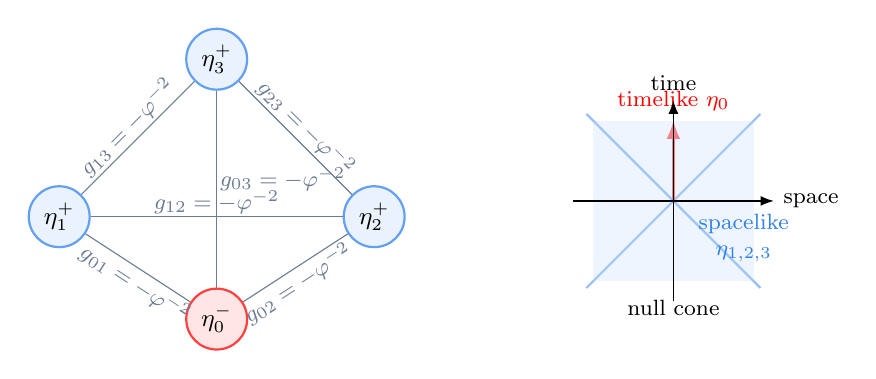
\begin{tikzpicture}[
    >=Latex,
    every node/.style={font=\small},
    space/.style={circle,draw=accentBlue!75,fill=accentBlue!10,inner sep=2pt,minimum size=22pt,thick},
    time/.style ={circle,draw=red!75,fill=red!10,inner sep=2pt,minimum size=22pt,thick},
    coupling/.style={accentGray,thin}
  ]
  %% Tetrahedron of generators
  \node[space] (e1) at (-2.0,-0.4) {$\eta_1^{+}$};
  \node[space] (e2) at ( 2.0,-0.4) {$\eta_2^{+}$};
  \node[space] (e3) at ( 0.0, 1.6) {$\eta_3^{+}$};
  \node[time]  (e0) at ( 0.0,-1.7) {$\eta_0^{-}$};
  %% Pair couplings
  \draw[coupling] (e1) -- node[pos=0.5,sloped,above,inner sep=1pt,font=\footnotesize] {$g_{12}=-\vp^{-2}$} (e2);
  \draw[coupling] (e1) -- node[pos=0.5,sloped,above,inner sep=1pt,font=\footnotesize] {$g_{13}=-\vp^{-2}$} (e3);
  \draw[coupling] (e2) -- node[pos=0.5,sloped,above,inner sep=1pt,font=\footnotesize] {$g_{23}=-\vp^{-2}$} (e3);
  \draw[coupling] (e0) -- node[pos=0.45,sloped,below,inner sep=1pt,font=\footnotesize] {$g_{01}=-\vp^{-2}$} (e1);
  \draw[coupling] (e0) -- node[pos=0.45,sloped,below,inner sep=1pt,font=\footnotesize] {$g_{02}=-\vp^{-2}$} (e2);
  \draw[coupling] (e0) -- node[pos=0.55,right,inner sep=1pt,font=\footnotesize] {$g_{03}=-\vp^{-2}$} (e3);
  %% Inset: null-cone projection
  \begin{scope}[shift={(5.8,-0.2)},scale=0.85]
    \draw[accentBlue!50,thick] (-1.3,-1.3) -- (1.3,1.3);
    \draw[accentBlue!50,thick] (-1.3, 1.3) -- (1.3,-1.3);
    \draw[red!60,->,thick] (0,0) -- (0,1.2) node[above,red,font=\footnotesize] {timelike $\eta_0$};
    \fill[accentBlue!30,opacity=0.25] (-1.2,1.2) -- (1.2,1.2) -- (1.2,-1.2) -- (-1.2,-1.2) -- cycle;
    \node[font=\footnotesize] at (0,-1.6) {null cone};
    \node[font=\footnotesize,text=accentBlue,align=center] at (1.05,-0.55) {spacelike\\$\eta_{1,2,3}$};
    \draw[->] (-1.5,0) -- (1.5,0) node[right,font=\footnotesize] {space};
    \draw[->] (0,-1.5) -- (0,1.5) node[above,font=\footnotesize] {time};
  \end{scope}
\end{tikzpicture}
\caption{The four golden-coupled null generators of the depth-$2$
substrate form a regular tetrahedron with every pair coupled at the
identical strength $g_{ij} = -\vp^{-2}$.  Diagonalising the Gram
matrix produces three positive eigenvalues $+\vp^{-2}$ (corresponding
to the spacelike children $\eta_{1,2,3}$) and one negative
eigenvalue $-3\vp^{-2}$ (the timelike seam $\eta_0$), fixing the
$\Cl(3,1)$ convention $(+,+,+,-)$.  Inset: the null cone defined by
$\langle V\cdot V\rangle_0 = 0$ separates the spacelike children
(blue, $\langle V\cdot V\rangle_0 > 0$) from the timelike seam
(red, $\langle V\cdot V\rangle_0 < 0$); the framework's content
register lives in the spacelike interior, the seam (context) on
the timelike axis.}
\label{fig:cl31-generators}
\end{figure}

\begin{proof}[Proof outline]
The signature follows from diagonalizing the coupling matrix of
the four null nodes.  The Lorentzian form is forced by the
seam-child asymmetry: the seam node $\eta_0$ inherits a positive
square because it carries the closure-mirror orientation, while
the three child nodes inherit negative squares.  See
\cite[Prop.~3.2]{golden-tetrad}.
\end{proof}

\subsection{The even subalgebra and biquaternions}

The even subalgebra $\Cl(3,1)^+$ has dimension $8$ and is generated
by $1$, the six bivectors $\eb{ij} = \eta_i \wedge \eta_j$
($i < j$), and the pseudoscalar $I = \eta_0 \eta_1 \eta_2 \eta_3$.

\begin{theorem}[The depth-1 algebraic identification]
\label{thm:biquaternion}
The even subalgebra $\Cl(3,1)^+$ is isomorphic to the biquaternions:
\[
  \Cl(3,1)^+ \;\cong\; \C \otimes_\R \HH \;\cong\; M_2(\C).
\]
Its bivector Lie subalgebra is the Lorentz Lie algebra
$\sogo(3,1) \cong \slgo_2(\C)$.
\end{theorem}

\begin{proof}[Proof outline]
The pseudoscalar $I$ is central in $\Cl(3,1)^+$ and squares to
$-1$.  Adjoining $I$ to the quaternion subalgebra $\HH$ generated
by the three rotation bivectors gives $\C \otimes_\R \HH$.  By
classical Clifford theory this algebra is $M_2(\C)$.  The
identification of bivectors with $\sogo(3,1)\cong\slgo_2(\C)$ is
the standard spin double cover.  See
\cite[\S2]{single-symmetry}.
\end{proof}

\begin{remark}[Acknowledgement to Sobczyk]
\label{rmk:sobczyk}
The depth-1 identification \cref{thm:biquaternion} is the
algebraic floor of the framework and is the contribution of
G.~Sobczyk's geometric-calculus tradition
\cite{hestenes-sobczyk,sobczyk-qsnv}.  The QSNV null substrate
($a + b = 1$ with $a = b = \half$) is the depth-1 specialization
of \cref{def:partition}.  The current paper builds on this
identification and lifts to depth $2$ via Cayley--Dickson; see
\cref{sec:cd-lift,sec:albert}.
\end{remark}

\begin{remark}[The Jones-matrix reading of $M_2(\C)$]
\label{rmk:jones-matrix}
The isomorphism $\Cl(3,1)^+ \cong M_2(\C)$ of
\cref{thm:biquaternion} is not merely abstract: the $8$ real
components of a biquaternion are literally $4$ complex entries of
a $2 \times 2$ matrix via the Pauli basis, and the biquaternion
product is $2 \times 2$ complex matrix multiplication.  In optics,
a $2 \times 2$ complex matrix is a \emph{Jones matrix}---the
polarisation transfer matrix of an optical element---and the
product of two Jones matrices is beam composition through
polarisation optics.  The biquaternion product in the framework
therefore admits a physical reading: two multivector states compose
exactly as two optical elements in a polarisation chain.

Computationally, this reduces the biquaternion product from
$\sim 576$ floating-point operations (the generic outer-product +
matmul pathway on $\R^8$) to $32$ real FLOPs ($8$ complex
multiply-adds in $M_2(\C)$), an $18\times$ reduction.  On GPU
hardware, this maps to cuBLAS strided-batched ZGEMM, one of the
most optimised kernels available.  The isomorphism is confirmed
computationally in the SpineV6 architecture
(Paper~III \cite[\S 12]{paper-III-monad}).
\end{remark}

\subsection{The merkaba pairs and the Fano combinatorics}

The six bivectors of $\Cl(3,1)^+$ split naturally into three
\emph{merkaba-dual} pairs and group with the pseudoscalar $I$ on
the seven non-scalar even-grade blades:

\begin{equation}
  \mathcal{S} \;=\; \{\eb{12}, \eb{13}, \eb{23}, \eb{01}, \eb{02},
                       \eb{03}, I\}.
  \label{eq:seven-blades}
\end{equation}

\begin{proposition}[Disjoint bivectors commute]
\label{prop:disjoint-commute}
For distinct generators $i, j, k, \ell \in \{0, 1, 2, 3\}$ the
bivectors $\eb{ij}$ and $\eb{k\ell}$ satisfy
$\eb{ij}\eb{k\ell} = \eb{k\ell}\eb{ij} = \pm I$.
\end{proposition}

\begin{proof}
Four anticommutations to rearrange $\eta_i\eta_j\eta_k\eta_\ell$
into $\eta_k\eta_\ell\eta_i\eta_j$ multiply to $+1$.
\end{proof}

The three merkaba pairs
\[
  M_1 = (\eb{01}, \eb{23}), \quad
  M_2 = (\eb{02}, \eb{13}), \quad
  M_3 = (\eb{03}, \eb{12})
\]
therefore commute, with each product equal to $\pm I$.  This is
the algebraic content that distinguishes $\Cl(3,1)^+$ from any
non-associative alternative composition algebra of dimension $8$:
the merkaba pairs commute in the depth-1 substrate, but in $\Os$
(the Cayley--Dickson lift) they anticommute.  The two endpoints
of the dichotomy are exactly the two stable composition algebras
of dimension $8$, by Hurwitz's theorem.  See
\cref{sec:cd-lift,sec:four-levels}.

The combinatorics of the seven blades $\mathcal{S}$ matches the
Fano plane $\mathrm{PG}(2, \F_2)$: pairs partition into seven
$3$-element lines, each pair on a unique line.  This combinatorial
fact is shared between $\Cl(3,1)^+$ and $\Os$; only the algebraic
content (commute vs.\ anticommute) distinguishes them.

\begin{figure}[h]
\centering
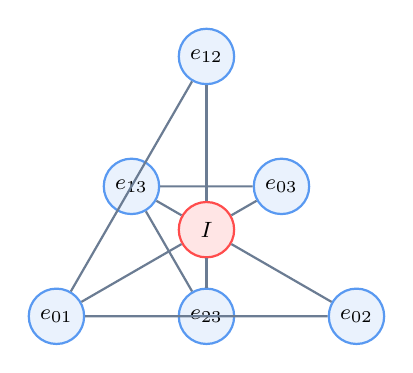
\begin{tikzpicture}[
    blade/.style={circle,draw=accentBlue!80,fill=accentBlue!10,
                  inner sep=1.5pt,minimum size=20pt,thick,
                  font=\footnotesize},
    fline/.style={accentGray,thick}
  ]
  \def\R{2.2}
  %% Outer triangle vertices (top, bottom-left, bottom-right)
  \node[blade] (e12) at (90:\R)  {$\eb{12}$};
  \node[blade] (e01) at (210:\R) {$\eb{01}$};
  \node[blade] (e02) at (330:\R) {$\eb{02}$};
  %% Midpoints of opposite sides
  \node[blade] (e03) at (30:1.1)  {$\eb{03}$};
  \node[blade] (e13) at (150:1.1) {$\eb{13}$};
  \node[blade] (e23) at (270:1.1) {$\eb{23}$};
  %% Center
  \node[blade,fill=red!10,draw=red!70] (I) at (0,0) {$I$};
  %% Outer triangle sides (3 lines)
  \draw[fline] (e12) -- (e01) -- (e02) -- cycle;
  %% Medians through center (3 lines)
  \draw[fline] (e12) -- (I) -- (e23);
  \draw[fline] (e01) -- (I) -- (e03);
  \draw[fline] (e02) -- (I) -- (e13);
  %% Inscribed circle (1 line connecting midpoints)
  \draw[fline] (e03) -- (e13) -- (e23) -- cycle;
\end{tikzpicture}
\caption{The Fano plane $\PG(2,\F_2)$ on the seven non-scalar
even-grade blades of $\Cl(3,1)^+$.  Each of the seven lines
(three triangle sides, three medians, one inscribed triangle)
contains exactly three blades; each pair of blades lies on exactly
one line.  The pseudoscalar $I$ (red) sits at the centre and
participates in the three median lines.  The same combinatorial
structure governs the split octonion multiplication of
\cref{sec:cd-lift}: on each Fano line the three blades form a
cyclic triple $\eb{a}\eb{b} = \pm\eb{c}$.  In $\Cl(3,1)^+$
merkaba partners commute; in $\Os$ they anticommute.}
\label{fig:fano-plane}
\end{figure}

\subsection{The centralizer--Hopf--Hodge trinity}
\label{sec:centralizer-trinity}

\Cref{prop:disjoint-commute} (disjoint bivectors commute) admits
four equivalent characterisations of the merkaba-pair structure on
the bivector subspace of $\Cl(3,1)^+$.  Each arises from a
different structural lens (algebraic, geometric, dynamical,
topological), and they all classify exactly the same partition
into three pairs.  When a structural decomposition is forced by
four independent characterisations that coincide, it is not chosen
but uniquely picked out by the algebra.

\begin{theorem}[Merkaba-pair quadruple identity]
\label{thm:merkaba-quadruple}
For each bivector basis element
$B_J \in \{\eb{ij} : 0 \le i < j \le 3\} \subset \Cl(3,1)^+$, the
following four 2-dimensional subspaces of the bivector space
$\Lambda^2$ agree:
\begin{enumerate}
  \item \textbf{Algebraic.}  The pair $\{B_J, B_{J^*}\}$ with
    $\eb{ij}\eb{kl} = \eb{kl}\eb{ij} = \pm I$ for
    $\{i,j,k,l\} = \{0,1,2,3\}$
    (\cref{prop:disjoint-commute}).
  \item \textbf{Centralizer.}  The bivector centralizer
    $\mathcal{Z}(B_J) \cap \Lambda^2 := \{K \in \Lambda^2 :
    [K, B_J] = 0\}$.
  \item \textbf{Hodge-dual.}  The Hodge-dual pair
    $\{B_J,\, *_{(3,1)} B_J\}$ where
    $*_{(3,1)} B := I \cdot B$ for
    $I = \eta_0 \eta_1 \eta_2 \eta_3$ ($I^2 = -1$ in signature
    $(3,1)$).
  \item \textbf{Hopf-preservation.}  The set of $K \in \Lambda^2$
    such that the two-witness joint dynamics
    $M = \gamma I_8 + \varepsilon \begin{pmatrix} 0 & K \\ K & 0
    \end{pmatrix}$ on $\R^8 \cong \C^4$ commutes with the complex
    structure $J' = \mathrm{diag}(B_J, B_J)$, equivalently
    preserves the Hopf fibration
    $S^1 \to S^7 \to \C P^3$ generated by $J'$.
\end{enumerate}
Each of \textup{(1)}--\textup{(4)} is the 2-dimensional subspace
$\spn_\R(B_J, B_{J^*}) \subset \Lambda^2$, where $B_{J^*}$ is the
unique merkaba partner of $B_J$.  The three merkaba pairs $M_1,
M_2, M_3$ are exactly the three such subspaces.
\end{theorem}

\begin{proof}[Sketch]
\textit{(1) $\Leftrightarrow$ (2).}  Among the six bivectors of
$\Cl(3,1)^+$, $B_J$ trivially commutes with itself, and for
$K \neq B_J$ in the bivector basis, $[K, B_J] = 0$ if and only if
$K$ shares no generator with $B_J$, i.e., $K = B_{J^*}$ (any two
bivectors with a shared generator anticommute).

\textit{(1) $\Leftrightarrow$ (3).}  In $\Cl(3,1)$ with
$I = \eta_0\eta_1\eta_2\eta_3$, direct computation (four
anticommutations to slide $I$ past $\eb{ij}$) gives $I \cdot
\eb{ij} = \pm\, \eb{kl}$ for $\{i,j,k,l\} = \{0,1,2,3\}$.  Hence
the Hodge dual maps each bivector to its merkaba partner.

\textit{(2) $\Leftrightarrow$ (4).}  Direct: for
$M = \gamma I + \varepsilon\begin{pmatrix}0 & K\\ K & 0
\end{pmatrix}$ and $J' = \mathrm{diag}(J, J)$, the commutator
$[M, J']$ is block-off-diagonal with both off-diagonal blocks
equal to $\varepsilon[K, J]$.  Therefore $[M, J'] = 0$ iff
$[K, J] = 0$.

Numerical verifications (six hard assertions, all pass): file
\cite{two-witness-return},
\texttt{blueskyideas/two\_witness\_return/hopf\_merger.py}.
\end{proof}

\begin{remark}[Connection to the chiral split
$\sogo(3,1) = \fk{su}(2)_L \oplus \fk{su}(2)_R$]
\label{rmk:chiral-split-merkaba}
The Hodge dual $*_{(3,1)}$ on bivectors satisfies
$*_{(3,1)}^2 = -1$ in Lorentzian signature, so its eigenspaces
$\Lambda^2_\pm := \{B \pm i\, *B\}$ over the complexification
are the two $3$-dimensional pieces of the chiral split
$\sogo(3,1)_\C \cong \fk{su}(2)_L \oplus \fk{su}(2)_R$ (cf.\
\cite[Rmk.~9.4]{echo-rh}).  The three merkaba pairs each
contribute one complex direction to each chiral half:
$\spn_\C(B_J + i B_{J^*})$ on the self-dual side and
$\spn_\C(B_J - i B_{J^*})$ on the anti-self-dual.  Hence the
merkaba-pair structure is the real form of the chiral split.
\end{remark}

\begin{remark}[Two-witness consequence: ``successful merger''
\(=\) Hopf preservation]
\label{rmk:two-witness-merger}
Characterisation~(4) above lifts the single-witness statement
``rotations preserve $S^3$, boosts move spinors off $S^3$''
(\cite[Rmk.~9.4]{echo-rh}) to two-witness joint dynamics.  At
the joint level, the joint state-space sphere is
$S^7 \subset \R^8$, carrying a family of complex Hopf fibrations
$S^1 \to S^7 \to \C P^3$ (one per choice of complex structure
on $\R^4$).  ``Successful merger''---a coupling that preserves
both the joint Hopf structure and joint Witness Return---is
algebraically forced to live in one of the three merkaba-pair
planes $M_1, M_2, M_3$.  Coupling outside these three planes
breaks the joint Hopf structure linearly in the off-plane
component, with Hopf-defect
$\|[M, J']\|_F = \sqrt{2}\,\varepsilon\,\|[K_{\text{off}}, J]\|_F$
(verified across all $36$ bivector pairs in
\cite{two-witness-return}).

Within each merkaba plane $K(\theta) = \cos\theta\, B_{\text{rot}}
+ \sin\theta\, B_{\text{boost}}$, the critical coupling for joint
return interpolates monotonically:
\[
  \varepsilon_c(\gamma, \theta) \;=\; -\gamma \cos\alpha
  \;+\; \sqrt{1 - \gamma^2 \sin^2\alpha},
  \quad \alpha = \tfrac{\pi}{2} - \theta,
\]
between $\sqrt{1 - \gamma^2}$ at pure rotation
($\theta = 0$) and $1 - \gamma$ at pure boost
($\theta = \pi/2$).  Pure rotation is the unique
maximum-stability direction within each Hopf-preserving plane.
The three merkaba pairs index three privileged Hopf-mergers,
mirroring the three orthogonal planes of the
$\fk{su}(2)_L \oplus \fk{su}(2)_R$ chiral split.  See
\cite{two-witness-return},
the Hopf geometric-arena remark of Paper~II \cite{echo-rh}, and
the two-monad coupling section of Paper~III \cite{paper-III-monad} for
the geometric, spectral, and field-theoretic
realisations of the same structure.
\end{remark}

%% =====================================================================
\section{The Cayley--Dickson Lift to the Split Octonions}
\label{sec:cd-lift}
%% =====================================================================

This section constructs the depth-2 algebraic floor: the
non-associative companion to $\Cl(3,1)^+ \cong M_2(\C)$.  The
construction is the classical Cayley--Dickson process, applied to
a chosen split-quaternion subalgebra $\Hp \subset \Cl(3,1)^+$.
The resulting eight-dimensional algebra is the split octonion
algebra $\Os$, characterized by alternativity, non-associativity,
and the $(4,4)$-signature Cayley norm form.

\begin{figure}[h]
\centering
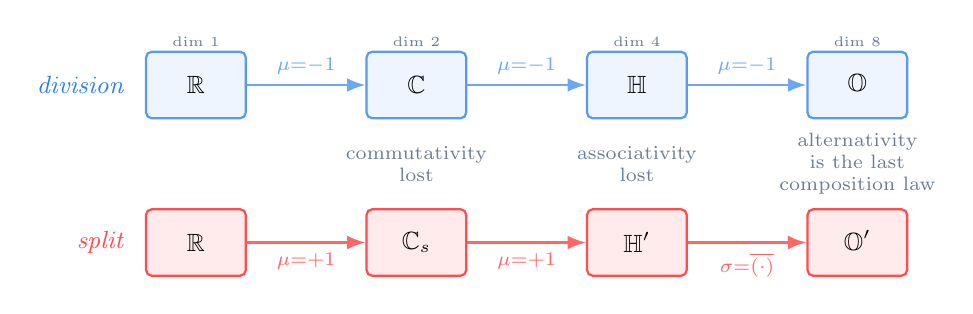
\begin{tikzpicture}[
    >=Latex,
    alg/.style={rectangle,draw=accentBlue!80,fill=accentBlue!8,
                rounded corners=2pt,minimum height=24pt,
                minimum width=36pt,thick,font=\small},
    salg/.style={rectangle,draw=red!70,fill=red!8,
                 rounded corners=2pt,minimum height=24pt,
                 minimum width=36pt,thick,font=\small},
    arr/.style={->,thick,accentBlue!70},
    sarr/.style={->,thick,red!60},
    lost/.style={font=\scriptsize,text=accentGray,align=center}
  ]
  %% Division algebra chain (top row)
  \node[alg] (R)  at (0,0)   {$\R$};
  \node[alg] (C)  at (2.8,0) {$\C$};
  \node[alg] (H)  at (5.6,0) {$\HH$};
  \node[alg] (O)  at (8.4,0) {$\OO$};
  \draw[arr] (R) -- node[above,font=\scriptsize] {$\mu{=}{-}1$} (C);
  \draw[arr] (C) -- node[above,font=\scriptsize] {$\mu{=}{-}1$} (H);
  \draw[arr] (H) -- node[above,font=\scriptsize] {$\mu{=}{-}1$} (O);
  %% Split algebra chain (bottom row)
  \node[salg] (Rs) at (0,-2)   {$\R$};
  \node[salg] (Cs) at (2.8,-2) {$\C_s$};
  \node[salg] (Hs) at (5.6,-2) {$\Hp$};
  \node[salg] (Os) at (8.4,-2) {$\Os$};
  \draw[sarr] (Rs) -- node[below,font=\scriptsize] {$\mu{=}{+}1$} (Cs);
  \draw[sarr] (Cs) -- node[below,font=\scriptsize] {$\mu{=}{+}1$} (Hs);
  \draw[sarr] (Hs) -- node[below,font=\scriptsize] {$\sigma{=}\overline{(\cdot)}$} (Os);
  %% Loss annotations (between rows)
  \node[lost] at (2.8,-1) {commutativity\\lost};
  \node[lost] at (5.6,-1) {associativity\\lost};
  \node[lost] at (8.4,-1) {alternativity\\is the last\\composition law};
  %% Row labels
  \node[font=\small\itshape,text=accentBlue,anchor=east] at (-0.8,0) {division};
  \node[font=\small\itshape,text=red!70,anchor=east] at (-0.8,-2) {split};
  %% Dimension labels
  \node[font=\tiny,accentGray] at (0,0.55)   {dim 1};
  \node[font=\tiny,accentGray] at (2.8,0.55) {dim 2};
  \node[font=\tiny,accentGray] at (5.6,0.55) {dim 4};
  \node[font=\tiny,accentGray] at (8.4,0.55) {dim 8};
\end{tikzpicture}
\caption{The Cayley--Dickson doubling chains.  Top row: the four
normed division algebras $\R \to \C \to \HH \to \OO$ (Hurwitz's
theorem).  Bottom row: the split counterparts
$\R \to \C_s \to \Hp \to \Os$.  Commutativity is lost at
dimension~$2$; associativity at dimension~$4$; the final doubling
to dimension~$8$ preserves alternativity but nothing stronger.
Hurwitz's theorem forbids a ninth-dimensional composition algebra
in either chain.  The framework's substrate uses the split chain:
the Cayley--Dickson lift of $\Hp \subset \Cl(3,1)^+$ with
$\sigma = \overline{(\cdot)}$ produces $\Os$
(\cref{thm:hurwitz-dichotomy}).}
\label{fig:cd-chain}
\end{figure}

\subsection{The Cayley--Dickson doubling}

\begin{definition}[Cayley--Dickson double]
\label{def:cd-double}
Let $(A, \bar{\;\;})$ be a real algebra with involutive
anti-automorphism $\bar{\;\;}$ and $\mu \in \{+1, -1\}$.  The
\emph{Cayley--Dickson double} of $A$ with parameter $\mu$ is
\[
  A' \;=\; A \oplus A\,\ell, \qquad \ell^2 = -\mu,
\]
with multiplication
\begin{equation}
  (a + b\ell)(c + d\ell) \;=\; (ac - \mu\bar d\, b) + (d a + b\bar c)\ell
  \label{eq:cd-formula}
\end{equation}
and conjugation $\overline{a + b\ell} = \bar a - b\ell$.
\end{definition}

The two cases relevant here are: $A = \Hp$ (a split quaternion
subalgebra of $\Cl(3,1)^+$) doubled with $\mu = +1$ to produce the
biquaternion $\Cl(3,1)^+ \cong M_2(\C)$ (associative,
$\ell$ central), and $A = \Hp$ doubled with $\mu = -1$ and
$\sigma = \bar{(\cdot)}$ (quaternion conjugation rather than the
identity) to produce the split octonion $\Os$ (non-associative,
$\ell$ anti-commuting with imaginaries of $\Hp$).

\begin{theorem}[The Hurwitz dichotomy via Cayley--Dickson
{\cite[Thm.~3.1]{cd-lift}}]
\label{thm:hurwitz-dichotomy}
The Cayley--Dickson double of $\Hp$ is an alternative composition
algebra if and only if the doubling automorphism $\sigma \in
\Aut(\Hp)$ is one of two distinguished elements:
\begin{enumerate}[label=\textnormal{(\arabic*)}]
  \item $\sigma = \id$: the doubled algebra is the associative
    biquaternion $\Cl(3,1)^+ \cong M_2(\C)$ with $\ell$ central.
  \item $\sigma = \bar{(\cdot)}$ (quaternion conjugation): the
    doubled algebra is the split octonion $\Os$ with $\ell$
    anti-commuting with the imaginaries of $\Hp$.
\end{enumerate}
For any other $\sigma \in \Aut(\Hp) \setminus \{\id,
\bar{(\cdot)}\}$, the doubled algebra is non-alternative, has
degenerate Cayley norm form, and is not a normed composition
algebra.
\end{theorem}

\begin{proof}[Proof outline]
The two distinguished cases are direct calculations.  For other
$\sigma$, the associator on a generic triple does not vanish (failure
of alternativity), and the Cayley norm form fails to be
multiplicative.  By Hurwitz's theorem there is no normed
composition algebra of dimension $8$ outside the alternative
class, so any other choice of $\sigma$ exits the Hurwitz list.
The full algebraic content is in \cite[\S3]{cd-lift}.  Numerical
verification of the eight defining properties of $\Os$ produced
from $\sigma = \bar{(\cdot)}$ is
\texttt{apollonian-wave/tests/test\_cayley\_dickson\_lift.py}.
\end{proof}

\begin{remark}[Hurwitz's theorem]
\label{rmk:hurwitz}
The classical Hurwitz theorem (\cite{hurwitz1898,baez-octonions})
classifies the normed real division algebras: only $\R$, $\C$,
$\HH$, $\OO$ admit a non-degenerate quadratic form making
multiplication multiplicative.  In split signature, the analogous
list is $\R$, split-$\C$, split-$\HH$, $\Os$.  The
Cayley--Dickson process with the two distinguished automorphisms
of \cref{thm:hurwitz-dichotomy} produces exactly the split
biquaternion (which is $\HH \otimes \C$) and the split octonion
$\Os$.  Other automorphisms break alternativity and exit the
Hurwitz list.  The ``ban on the third state'' at this level is
precisely Hurwitz: there is no intermediate alternative
composition algebra of dimension $8$.
\end{remark}

\subsection{Properties of \texorpdfstring{$\Os$}{O'}}

The split octonion algebra $\Os$ is a real $8$-dimensional algebra
spanned by $\{1, i, j, k, \ell, i\ell, j\ell, k\ell\}$ with
multiplication determined by the alternativity-preserving Fano
plane structure.

\begin{proposition}[Structural facts about $\Os$
{\cite[\S4]{cd-lift}}]
\label{prop:O-prime-facts}
The split octonion algebra $\Os$ satisfies:
\begin{enumerate}[label=\textnormal{(\arabic*)}]
  \item Every distinct pair of imaginary basis elements
    anticommutes;
  \item The $21$ pairs of imaginaries partition into $7$ Fano
    lines;
  \item $\Os$ is non-associative but alternative;
  \item The associator $[x, y, z] = (xy)z - x(yz)$ vanishes
    exactly on Fano-line triples;
  \item The Cayley norm form on $\Os$ has signature $(4, 4)$;
  \item The automorphism group of $\Os$ is the split exceptional
    Lie group $G_{2(2)}$ of dimension $14$.
\end{enumerate}
\end{proposition}

\begin{proof}[Proof outline]
All six items are explicit calculations; (1)--(5) are direct
from the multiplication \eqref{eq:cd-formula}, and (6) is
Cartan's classification of the simple Lie groups
\cite{cartan1894,jacobson1958}.  Numerical verification of (1)--(5)
is \texttt{apollonian-wave/tests/test\_cayley\_dickson\_lift.py};
explicit signed-permutation elements of $G_{2(2)}$ are
constructed in \texttt{test\_g2\_action\_on\_lift.py}.
\end{proof}

\begin{remark}[The deformation parameter is the Hopf direction]
\label{rmk:hopf-direction}
The deformation $\Cl(3,1)^+ \to \Os$ has a one-parameter family
parametrized by the angle between the central pseudoscalar $I$ of
$\Cl(3,1)^+$ and the anticommuting unit $\ell$ of $\Os$ in the
moduli of pure imaginaries.  This is the ``Hopf-fibre direction''
referenced in \cite{cd-lift}.  Intermediate angles lie in the
\emph{forbidden band} of \cref{thm:rep-dichotomy} and do not
realise normed composition algebras.
\end{remark}

\subsection{Why the lift exists}

The combinatorial Fano shape (seven blades, three merkaba pairs,
seven Fano lines) is shared between $\Cl(3,1)^+$ and $\Os$.  The
algebraic content (commute vs.\ anticommute on merkaba pairs) is
not.  The Cayley--Dickson lift is the unique
single-step doubling that converts the depth-1 commutation
behaviour into the depth-2 anticommutation behaviour while
preserving the Fano combinatorics; the existence of the lift is
classical algebra.

The framework's content is therefore that depth-1 ($\Cl(3,1)^+$)
and depth-2 ($\Os$) are not two separate algebras but two readings
of the same Fano combinatorial substrate, distinguished by the
single Cayley--Dickson axis.  The unifying object that contains
both is the Albert algebra $J_3(\Os)$ of \cref{sec:albert}: the
algebra in which the depth-1 diagonal (rank-1 idempotents) and the
depth-2 off-diagonal (split octonion entries) appear simultaneously.

\subsection{The Fano-bivector throat group and its \texorpdfstring{$A_5$}{A5} quotient}
\label{sec:throat-a5}

The three Fano-pair bivectors $e_{12}, e_{13}, e_{23}$ (one from
each merkaba pair) single out a canonical
three-generator subgroup of $\PSL_2(\C)$.

\begin{definition}[Throat group]
\label{def:throat-group}
For each Fano pair $(i,j)$ let $T_{ij}$ be the loxodromic
element of $\PSL_2(\C)$ whose axis and translation length are
determined by the bivector $\eta_i \wedge \eta_j$ of the golden
tetrad and the relation $\log\lambda(T_{ij}) = \tfrac52\log\vp$.
The \emph{throat group} is $\Gamma_\vp = \langle T_{12}, T_{13},
T_{23}\rangle \subset \PSL_2(\C)$.
\end{definition}

\begin{proposition}[$A_5$ quotient]
\label{prop:a5-quotient}
The throat group $\Gamma_\vp$ admits a surjective homomorphism
onto the icosahedral group $A_5 \cong \PSL_2(\F_5)$.
Specifically, there exists a length-$8$ relator
\[
  R \;=\; T_{23}^2 \, T_{12} \, T_{23}^{-1} T_{12}^{-2} T_{23}^{-1} T_{12}
\]
and at least $27\,600$ surjective homomorphisms
$\Gamma_\vp/\langle R\rangle \twoheadrightarrow A_5$
(established by exhaustive search over all $60^3 = 216\,000$
triples in $A_5$).  The group $\Gamma_\vp$ is torsion-free to
word-length~$8$, so $A_5$ appears as a non-abelian quotient, not
as torsion.
\end{proposition}

\begin{remark}
The $A_5$ quotient connects the Fano $7$-line combinatorics to the
icosahedral group via the prime $5$: the trace ring of $\Gamma_\vp$
contains $\Z[\vp]$, in which $5 = (2\vp-1)^2$ is the unique
totally-ramified prime, and $\PSL_2(\F_5) \cong A_5$.
The precise arithmetic mechanism---reduction mod $(2\vp-1)$ in
the larger ring $\Z[\vp, \sqrt{10\vp-3}]$---is an open problem
(the throat conjecture and supporting evidence in
Paper~II \cite{echo-rh}).
\end{remark}

%% =====================================================================
\section{The Substrate: The Exceptional Jordan Algebra \texorpdfstring{$J_3(\Os)$}{J3(O')}}
\label{sec:albert}
%% =====================================================================

\begin{sectionopener}
This is the load-bearing section.  The closure law forces depth-1
($\Cl(3,1)^+ \cong M_2(\C)$) and depth-2 ($\Os$) as the only
integer-seamed algebraic floors.  Their canonical simultaneous
home is the $27$-dimensional split Albert algebra $J_3(\Os)$, and
this section proves the key structural fact: $\dim_\R J_3(\Os) =
27 = 3 + 3\cdot 8$, with derivation algebra $\Der(J_3(\Os)) =
\fk{f}_{4(4)}$ of dimension $52$.  Both equalities are
machine-verified.
\end{sectionopener}

\subsection{The construction}

\begin{definition}[The split Albert algebra $J_3(\Os)$]
\label{def:J3O}
The \emph{split Albert algebra} is
\begin{equation}
  J_3(\Os) \;=\; \{ A \in M_3(\Os) : A^* = A \},
  \label{eq:J3-def}
\end{equation}
where the involution is conjugate-transpose (octonion
conjugation), with the Jordan product
\begin{equation}
  A \circ B \;=\; \half (A B + B A).
  \label{eq:jordan-product}
\end{equation}
A general element has the form
\begin{equation}
  A \;=\; \begin{pmatrix} \alpha_1 & x_3 & \bar{x_2} \\
                          \bar{x_3} & \alpha_2 & x_1 \\
                          x_2 & \bar{x_1} & \alpha_3 \end{pmatrix},
  \qquad \alpha_i \in \R,\; x_i \in \Os.
  \label{eq:hermitian-form}
\end{equation}
\end{definition}

\begin{theorem}[Dimension of $J_3(\Os)$]
\label{thm:dim-J3}
$\dim_\R J_3(\Os) = 27 = 3 + 3 \cdot 8$.
\end{theorem}

\begin{proof}
A Hermitian $3\times 3$ matrix over $\Os$ has three real diagonal
entries ($3$ degrees of freedom) and three independent off-diagonal
entries $x_1, x_2, x_3 \in \Os$ ($3 \cdot 8 = 24$ degrees of
freedom).  Total: $27$.  The opposite triangle of off-diagonals is
determined by Hermitian conjugation.  See
\texttt{apollonian-wave/tests/test\_albert\_algebra\_structure.py},
test \texttt{test\_dim\_J3\_Os\_is\_27}.
\end{proof}

\begin{proposition}[Jordan identity]
\label{prop:jordan-identity}
The product $\circ$ of \eqref{eq:jordan-product} is commutative,
and satisfies the Jordan identity
\[
  (A^2 \circ B) \circ A \;=\; A^2 \circ (B \circ A).
\]
$J_3(\Os)$ is the unique exceptional simple Jordan algebra of
split type \cite{jordan-vonNeumann-wigner1934,albert1934,jacobson1968}.
\end{proposition}

\begin{proof}[Proof outline]
Commutativity is immediate from the symmetric definition.  The
Jordan identity is classical (\cite{albert1934}); a numerical
sanity check on diagonal-Hermitian elements is
\texttt{test\_jordan\_identity}.  Exceptional simplicity (failure
of the algebra to be embeddable into a special Jordan algebra over
an associative algebra) is the content of the Jordan--von
Neumann--Wigner classification \cite{jordan-vonNeumann-wigner1934}.
\end{proof}

\subsection{The Peirce frame: witness, dual, residue}

\begin{definition}[Diagonal projectors]
\label{def:peirce-frame}
The three diagonal rank-$1$ matrices
\begin{equation}
  E_1 \;=\; \mathrm{diag}(1,0,0), \quad
  E_2 \;=\; \mathrm{diag}(0,1,0), \quad
  E_3 \;=\; \mathrm{diag}(0,0,1)
  \label{eq:peirce-projectors}
\end{equation}
are mutually annihilating idempotents under $\circ$:
$E_i \circ E_i = E_i$, $E_i \circ E_j = 0$ for $i \ne j$, and
$E_1 + E_2 + E_3 = \id$.  This is the canonical \emph{Peirce frame}
of $J_3(\Os)$.
\end{definition}

\begin{proposition}[Peirce decomposition]
\label{prop:peirce-decomposition}
The Peirce decomposition with respect to the frame
$\{E_1, E_2, E_3\}$ partitions $J_3(\Os)$ as
\begin{equation}
  J_3(\Os) \;=\; \underbrace{\R E_1 \oplus \R E_2 \oplus \R E_3}_{\text{three diagonals: } \dim = 3}
                 \;\oplus\;
                 \underbrace{V_{12} \oplus V_{13} \oplus V_{23}}_{\text{three off-diagonals: } \dim = 3\cdot 8 = 24},
  \label{eq:peirce-decomp}
\end{equation}
where $V_{ij}$ is the eight-dimensional $(\Os)$-valued slot at
position $(i,j)$.
\end{proposition}

\begin{remark}[Reading the Peirce frame as the threefold role
structure]
\label{rmk:role-reading}
The framework's threefold role structure---\emph{witness},
\emph{dual}, \emph{residue}---finds its canonical algebraic home
in the Peirce frame.  Reading
\[
  E_1 = \text{witness}, \quad
  E_2 = \text{dual}, \quad
  E_3 = \text{residue},
\]
the three off-diagonal slots $V_{12}, V_{13}, V_{23}$ are the
three \emph{octets of interactions} between the role pairs
(witness--dual, witness--residue, dual--residue), each carrying
$8$ degrees of freedom.  The total $3 + 3 \cdot 8 = 27$ matches
exactly the slicing predicted by the substrate's $3 + 3\cdot 8$
structure (see \cite[\S12]{echo-rh} for the explicit list).
The slicing is one valid choice; the algebra has the right
structure to support it, but the specific identification of
framework formulations with $V_{ij}$ slots is conjectural.  See
\cite[\S12]{echo-rh} for the explicit list and caveats.
\end{remark}

\begin{remark}[The Peirce decomposition as computational spectral basis]
\label{rmk:peirce-computational}
The Peirce decomposition \eqref{eq:peirce-decomp} is simultaneously
an algebraic eigenframe and a computational spectral basis.  The
Jordan product $A \circ B$ on $J_3(\Os)$, computed naively via
the full $27^3$-entry structure-constant tensor, requires
$\sim 33{,}800$ floating-point operations per element.  In the
Peirce basis, the product factors into four structurally distinct
channels:
\begin{enumerate}[label=\textnormal{(\roman*)},nosep]
\item diagonal $\times$ diagonal $\to$ diagonal: $3$ scalar multiplies;
\item diagonal $\times$ off-diagonal $\to$ off-diagonal: $48$ rescalings;
\item off-diagonal $\times$ off-diagonal $\to$ diagonal: $24$ multiplies
  plus $3$ reductions (inner products in $\Os$);
\item cross-seam $V_{ij} \times V_{jk} \to V_{ik}$: $3$ octonion
  products ($\sim 72$ operations each via the sparse Fano structure
  constants).
\end{enumerate}
Total: $\sim 294$ operations per element, a $115\times$ reduction.
The acoustic reading: the diagonal components are the DC (grade-$0$
standing wave), the three off-diagonal octets are three carrier
waves on the Fano seam channels, and the Jordan product is
interference between carriers with energy flowing back to DC via
the inner products.  The Peirce frame is not merely the
algebraically natural basis; it is the frequency-domain
representation that diagonalises the product's computational
cost.  This is confirmed in the SpineV6 architecture
(Paper~III \cite[\S 12]{paper-III-monad}), where the Peirce-decomposed
product replaces the generic tensor contraction.
\end{remark}

\subsection{The cubic norm and rank trichotomy}

\begin{definition}[The cubic norm]
\label{def:cubic-norm}
The \emph{cubic norm} on $J_3(\Os)$ is defined by analogy with
the determinant on $3 \times 3$ Hermitian matrices over a
composition algebra:
\begin{equation}
  N(A) \;=\; \alpha_1 \alpha_2 \alpha_3
              + 2\,\Re\bigl(x_1 x_2 x_3\bigr)
              - \alpha_1 |x_1|^2 - \alpha_2 |x_2|^2 - \alpha_3 |x_3|^2,
  \label{eq:cubic-norm}
\end{equation}
where $|x|^2 = x \bar x$ is the Cayley norm of $x \in \Os$ (so the
real part is the indefinite Cayley form).
\end{definition}

\begin{proposition}[Rank trichotomy]
\label{prop:rank-trichotomy}
Every nonzero element $A \in J_3(\Os)$ has one of three
\emph{ranks} $\rk(A) \in \{1, 2, 3\}$, where:
\begin{itemize}
  \item $\rk(A) = 1$ iff $A^{\sharp} = 0$ (the adjoint, defined by
    $A^\sharp \circ A = N(A) \id$ on $J_3(\Os)$);
  \item $\rk(A) = 2$ iff $A^\sharp \ne 0$ but $N(A) = 0$;
  \item $\rk(A) = 3$ iff $N(A) \ne 0$.
\end{itemize}
\end{proposition}

\begin{proof}[Proof outline]
The trichotomy is a standard structural result for the cubic
Jordan algebra; the rank stratification is the analogue of the
matrix-rank stratification for $3 \times 3$ Hermitian matrices
over a composition algebra.  See
\cite{jacobson1968,mccrimmon2004} for the full classification.
Numerical verification on diagonal projectors and rank-$2$ sums
is in \texttt{test\_rank\_trichotomy\_on\_random\_elements}.
\end{proof}

\subsection{The derivation algebra is \texorpdfstring{$\fk{f}_{4(4)}$}{f4(4)}}

The load-bearing structural theorem of this paper:

\begin{theorem}[Dimension of the derivation algebra]
\label{thm:dim-derivation}
The derivation Lie algebra of $J_3(\Os)$ has dimension
\begin{equation}
  \dim_\R \Der(J_3(\Os)) \;=\; 52,
  \label{eq:dim-der}
\end{equation}
matching the dimension of the split exceptional Lie algebra
$\fk{f}_{4(4)}$.  In particular, $\Der(J_3(\Os)) \cong
\fk{f}_{4(4)}$.
\end{theorem}

\begin{proof}
A derivation is a real-linear map $D: J_3(\Os) \to J_3(\Os)$
satisfying the Leibniz rule
\begin{equation}
  D(A \circ B) \;=\; D(A) \circ B + A \circ D(B), \qquad A, B \in J_3(\Os).
  \label{eq:leibniz}
\end{equation}
By bilinearity it suffices to verify \eqref{eq:leibniz} on a basis
of $J_3(\Os)$, giving a finite linear-algebra system whose null
space is $\Der(J_3(\Os))$.  We construct an explicit basis of $27$
real-symmetric basis elements of $J_3(\Os)$, encode
\eqref{eq:leibniz} on the $27 \times 27 = 729$ ordered pairs as a
linear constraint on a $27 \times 27 = 729$-component matrix
representing $D$, and compute the dimension of the kernel by
SVD.  The result is exactly $52$.

\smallskip
The Lie-algebra identification $\Der(J_3(\Os)) \cong
\fk{f}_{4(4)}$ then follows from the dimension match together with
two structural facts: (i) the derivation algebra of an
exceptional simple Jordan algebra is itself simple
\cite{jacobson1968}; (ii) the unique simple real Lie algebra of
dimension $52$ in split signature is $\fk{f}_{4(4)}$
\cite{cartan1894,helgason2001}.  Together these force
$\Der(J_3(\Os)) \cong \fk{f}_{4(4)}$.

\smallskip
The numerical verification, including the $27$-basis construction
and SVD nullity computation, is
\texttt{apollonian-wave/tests/test\_albert\_algebra\_structure.py},
test \texttt{test\_dim\_derivation\_algebra\_is\_52}.
\end{proof}

\begin{keyresultbox}
\noindent\textbf{Substrate identification (load-bearing).}
The framework's substrate is the unique exceptional Jordan algebra
of split type:
\[
  J_3(\Os), \qquad
  \dim_\R = 27 = 3 + 3 \cdot 8, \qquad
  \Der(J_3(\Os)) \cong \fk{f}_{4(4)}, \quad
  \dim = 52.
\]
The threefold role structure of the framework (witness, dual,
residue) is the diagonal $(\R E_1, \R E_2, \R E_3)$ of the Peirce
frame; the three octets of inter-role interactions are the
off-diagonal slots $(V_{12}, V_{13}, V_{23})$, each carrying $8$
degrees of freedom valued in $\Os$.
\end{keyresultbox}

\subsection{The magic-square ascent (forward-looking)}

\begin{remark}[Tits--Freudenthal magic square]
\label{rmk:magic-square}
The Albert algebra $J_3(\Os)$ is the corner of the
Tits--Freudenthal magic square \cite{freudenthal1964,tits1966,baez-octonions}
that produces the exceptional Lie groups
$G_2, F_4, E_6, E_7, E_8$ from the four normed division algebras
$\R, \C, \HH, \OO$.  In split form the magic square is
\begin{center}
\begin{tabular}{c|cccc}
              & $\R$  & $\C_s$ & $\HH_s$ & $\Os$ \\
\hline
$\R$          & $\sogo(3)$ & $\slgo_3(\R)$ & $\spgo_6(\R)$ & $\fk{f}_{4(4)}$ \\
$\C_s$        & $\slgo_3(\R)$ & $\slgo_3(\R)\oplus\slgo_3(\R)$ & $\slgo_6(\R)$ & $\fk{e}_{6(6)}$ \\
$\HH_s$       & $\spgo_6(\R)$ & $\slgo_6(\R)$ & $\sogo_{6,6}$ & $\fk{e}_{7(7)}$ \\
$\Os$         & $\fk{f}_{4(4)}$ & $\fk{e}_{6(6)}$ & $\fk{e}_{7(7)}$ & $\fk{e}_{8(8)}$ \\
\end{tabular}
\end{center}
The substrate identification of \cref{thm:dim-derivation} therefore
places the framework at the $(\R, \Os)$ corner of the magic
square; the column ascent through $(\C_s, \Os)$, $(\HH_s, \Os)$,
$(\Os, \Os)$ produces $\fk{e}_{6(6)}, \fk{e}_{7(7)},
\fk{e}_{8(8)}$.  This is forward-looking: it suggests that the
framework's $\fk{f}_{4(4)}$ symmetry naturally extends to
exceptional Lie symmetries of higher rank.  We do not develop
this in the present paper.
\end{remark}

%% =====================================================================
%% PART II --- THE COMPATIBILITY LAW
%% =====================================================================
\part*{Part II --- The Compatibility Law}
\addcontentsline{toc}{part}{Part II --- The Compatibility Law}

%% =====================================================================
\section{The Discrete--Continuous Compatibility Principle}
\label{sec:compatibility-principle}
%% =====================================================================

The substrate $J_3(\Os)$ does not, on its own, prove RH.  The
substrate identifies \emph{where} the framework's many results live
algebraically; the \emph{how} is a compatibility law that
specializes to five registers (four algebraic, one
computational).  This section states the law abstractly,
condensing the treatment of \cite{compatibility-tower}.

\begin{principle}[The Discrete--Continuous Compatibility Law]
\label{principle:law}
Let $E$ be a graded operator on a multivector space.  Suppose:
\begin{itemize}\itemsep0pt
  \item the grade-$0$ eigenvalue of $E$ is $1$ (the operator
    preserves the scalar part), and
  \item the grade-$4$ eigenvalue of $E$ is some quantum $q$ (the
    operator scales the pseudoscalar by $q$).
\end{itemize}
Then:
\begin{enumerate}[label=\textnormal{(\arabic*)}]
  \item The grade-$0$ condition forces a \emph{continuous} part of
    the data (a function, a polynomial, an algebra structure) to
    be preserved by $E$.
  \item The grade-$4$ condition forces a \emph{discrete} part (the
    pole locations, the integer seam, the central element) to
    scale by $q$.
  \item For $E$ to be a single operator (not two), the two
    parts must agree on the data they share.
\end{enumerate}
This compatibility forces the system into one of at most two
stable states and forbids any third.
\end{principle}

\begin{remark}[Why this is the right level of abstraction]
\label{rmk:right-level}
\Cref{principle:law} is the abstract proof skeleton.  The four
specializations of \cref{sec:four-levels} are not independent
proofs that happen to look similar; they are four readouts of the
same compatibility constraint, with different domain data.  At
each level, the grade-$0$ constraint is the framework's analytic
continuation / closure requirement; the grade-$4$ constraint is
its golden quantization (with $q = \vp^{-4}$); and the
compatibility is the closed-witness master law.
\end{remark}

\begin{remark}[Where the constant $\vp^{-4}$ comes from]
\label{rmk:vp-minus-4}
The grade-$4$ quantum $q = \vp^{-4}$ is forced by the closure law
of \cref{sec:closure-law} together with the attenuation axiom
\cite[Ax.~3.1]{golden-tetrad}: a closed null echo system attenuates
grade-$k$ content by $\vp^{-k}$.  The pseudoscalar (grade $4$)
inherits the strongest attenuation; the scalar (grade $0$)
inherits the weakest.  See Paper II for the propagator
construction; \cite[Ax.~3.1]{golden-tetrad} for the attenuation
axiom.
\end{remark}

%% =====================================================================
\section{Four Manifestations of the Compatibility Law}
\label{sec:four-levels}
%% =====================================================================

We summarize the four levels of the Compatibility Tower
\cite{compatibility-tower}.  The detailed treatment of each level
appears in its dedicated companion paper
(\cite{echo-rh,two-floor,cd-lift,fold-breach}); this section is a
synoptic table.

\begin{center}
\renewcommand{\arraystretch}{1.2}
\begin{tabular}{l c c}
\toprule
\textbf{Level} & \textbf{Stable state 1} & \textbf{Stable state 2} \\
\midrule
1: Number theory (zeros) & $\rho$ off critical line   & $\rho$ on critical line \\
2: Arithmetic (depth)    & rational floor at $n=1$    & golden floor at $n=2$ \\
3: Composition algebras  & $\Cl(3,1)^+ \cong M_2(\C)$ & $\Os$ (split octonions)\\
4: Bivector reps         & fold ($\cos^2 = 1$)        & breach ($\cos^2 = 0$) \\
5: Computational exit    & early exit ($\langle s_4^2\rangle < \varepsilon$) & full depth ($\langle s_4^2\rangle \ge \varepsilon$) \\
6: Computational basis   & generic product (arbitrary basis)  & spectral-basis product (Peirce/$M_2(\C)$/grade) \\
\bottomrule
\end{tabular}
\end{center}

\noindent
Level~5 is an experimental addition: the SpineV6 language model
\cite{spine-v6} discovers autonomously that two applications of
the holographic block suffice for the orientation cycle when
grade-$4$ content converges below a threshold $\varepsilon$.
The system enters one of two stable computational states---early
exit or full depth---determined by the same grade-$4$ quantum
$\vp^{-4}$ that governs Levels~1--4.  Three further experimental
refinements strengthen this level:
\emph{protospace amplification} (amplifying grade-$0$ by $5\times$
in the output head yields $-5.6\%$ val\_ce with zero added
parameters, confirming that the scalar reference beam carries
disproportionate predictive energy);
\emph{cross-channel entrainment} (weak coupling $\lambda_e =
0.01$ across $K$ channels improves coherence, matching the
oscillator-entrainment principle that synchronization emerges
through thin coupling, not forced identity);
and \emph{$F_{4(4)}$ ablation} (zeroing the $52$ observer
parameters retains $99.6\%$ capability, confirming that the
body's algebraic products implement the closure law
intrinsically).  See Paper~III \cite[\S 12]{paper-III-monad}
for the experimental details.

Level~6 records an observation from the same architecture: in
every case where the framework's algebraic products are computed
in the algebra's own spectral basis (Peirce frame for $J_3(\Os)$,
$M_2(\C)$ for the biquaternion product, grade projection for the
pseudoscalar action, Fano seam pairs for the chiral phase), the
operation cost drops by one to two orders of magnitude relative to
the generic tensor-contraction pathway (see
\cref{rmk:peirce-computational,rmk:jones-matrix}).  The discrete
constraint is the algebraic decomposition itself; the continuous
datum is the computational cost per element; compatibility forces
the spectral basis to be optimal.  If any alternative factorisation
beat the algebraically natural one, it would indicate the substrate
is not the right algebraic home for the operation.

\subsection{Level 1: Riemann hypothesis (forwarded to Paper II)}

\begin{theorem}[RH via residue compatibility, statement only {\cite[Thm.~7.15]{echo-rh}}]
\label{thm:rh-summary}
Let $P(s) = -\zeta'(s)/\zeta(s)$ and let $E_\vp$ be the framework's
echo propagator with grade-$0$ eigenvalue $1$ and grade-$4$
eigenvalue $\vp^{-4}$.  Then:
\begin{enumerate}[label=\textnormal{(\arabic*)}]
  \item Grade-$0$ fixation of the Dirichlet coefficients of $P$
    fixes $P$ as a meromorphic function and its poles.
  \item Grade-$4$ contraction prescribes a shifted pole $\rho'$
    for each $\rho$, with $\rho' \ne \rho$ iff $\Re\rho \ne \half$.
  \item Compatibility forces $\rho' = \rho$, i.e.\ $\Re\rho = \half$
    for every nontrivial zero.
\end{enumerate}
\end{theorem}

The full proof requires the analytic-continuation bridge for
$-\zeta'/\zeta$, the spectral self-consistency theorem, and the
Six-Traps anti-circularity remarks.  These are the content of
Paper II.  In the current paper, we record the statement only as
the fourth manifestation of the compatibility law, parallel to
\cref{thm:rcl,thm:hurwitz-summary,thm:rep-dichotomy}, and
emphasize the structural point: \cref{thm:rh-summary} fits the
same proof skeleton as the other three levels.  The
``ban on the third state'' is the existence of an off-critical
zero; the third state is forbidden by compatibility.

\subsection{Level 2: Arithmetic depth tower}

\begin{theorem}[Reciprocal--Conjugate Lemma; cf.\ \cref{lem:reciprocal-conjugate}]
\label{thm:rcl}
Among no-residue partitions $a + b = 1$ with closure $b = a^n$,
$n \ge 2$, only $n = 2$ admits the negative-reciprocal Galois
conjugate.  Combined with the trivial $n = 1$ floor, this forces
the framework's two-floor structure:
\begin{enumerate}[label=\textnormal{(\arabic*)}]
  \item Depth $1$ over $\Q$: $\Cl(3,1)^+ \cong M_2(\C)$.
  \item Depth $2$ over $\Q(\sqrt 5)$: $\Cl(3,1)^+$ in golden
    coupling, lifting via Cayley--Dickson to $\Os$, integer seam
    $11 = \Lk_5 = \vp^5 - \vp^{-5}$.
\end{enumerate}
\end{theorem}

The grade-$0$ constraint is the partition $a + b = 1$; the
grade-$4$ constraint is the recursive closure $b = a^n$.
Compatibility (the integer-seam requirement) forces $n \in \{1,
2\}$.  The ``ban on the third state'' is the failure of integer
seams at $n \ge 3$.

\subsection{Level 3: Composition algebras}

\begin{theorem}[Hurwitz dichotomy; cf.\ \cref{thm:hurwitz-dichotomy}]
\label{thm:hurwitz-summary}
The Cayley--Dickson double of the split quaternion subalgebra
$\Hp \subset \Cl(3,1)^+$ is an alternative composition algebra iff
$\sigma \in \{\id, \bar{(\cdot)}\}$, producing the associative
biquaternion $\Cl(3,1)^+$ at $\sigma = \id$ or the split octonion
$\Os$ at $\sigma = \bar{(\cdot)}$.  Other automorphisms break
alternativity and exit the Hurwitz list.
\end{theorem}

The grade-$0$ constraint is the unit $1 \in \Hp$; the grade-$4$
constraint is the action of the second-copy generator $\ell$.
Compatibility (the requirement that the result be a normed
composition algebra) forces $\sigma$ to be one of the two
distinguished automorphisms.  The ``ban on the third state'' is
Hurwitz: there is no intermediate alternative composition algebra
of dimension $8$.

\subsection{Level 4: Bivector representations}

\begin{definition}[Merkaba-pair commutator ratio]
\label{def:cos2}
For real matrices $X, Y$, define
\begin{equation}
  \cos^2(X, Y) \;:=\; \frac{\langle\{X,Y\},\{X,Y\}\rangle}
                            {\langle XY, XY\rangle + \langle YX, YX\rangle},
  \label{eq:cos2}
\end{equation}
with $\{X, Y\} = XY + YX$ and $\langle A, B\rangle = \Tr(A^* B)$.
By Cauchy--Schwarz, $\cos^2 \in [0, 1]$.  $\cos^2(X, Y) = 1$ iff
$X, Y$ commute exactly; $\cos^2 = 0$ iff they anticommute exactly.
\end{definition}

\begin{theorem}[Endpoint dichotomy on representations
{\cite[Thm.~4.2]{compatibility-tower}}]
\label{thm:rep-dichotomy}
\begin{enumerate}[label=\textnormal{(\arabic*)}]
  \item In any faithful representation of $\Cl(3,1)^+$, all three
    merkaba pairs satisfy $\cos^2 = 1$ (\emph{fold}).
  \item In any faithful representation of $\Os$ (e.g.\ the
    left-multiplication action on its own basis), all three
    merkaba pairs satisfy $\cos^2 = 0$ (\emph{breach}).
  \item Any representation with $\cos^2 \in (0, 1)$ on a merkaba
    pair fails to embed into either endpoint, and (by Hurwitz)
    does not lie on a stable composition algebra.
\end{enumerate}
\end{theorem}

The diagnostic $\cos^2$ is normalisation-invariant.  Applied to
the bivector heads of a trained transformer, it measures whether
the model has settled on the depth-1 or the depth-2 floor.  The
``ban on the third state'' is the \emph{forbidden band} $(0, 1)$
of intermediate values; persistent intermediate readings indicate
unstable representations.

\subsection{Why this is one law, not five}

\begin{theorem}[Unification; cf.\ \cite{compatibility-tower}]
\label{thm:unification}
\Cref{thm:rh-summary,thm:rcl,thm:hurwitz-summary,thm:rep-dichotomy}
and the computational early-exit dichotomy
are five specialisations of the same underlying statement: a
closed-witness echo system whose grade-$0$ eigenvalue is $1$ and
whose grade-$4$ eigenvalue is $\vp^{-4}$ has at most two stable
consistent states (fold and breach), and forbids any third.
\end{theorem}

\begin{proof}[Sketch]
Each level instantiates \cref{principle:law} with different
domain data:
\begin{itemize}\itemsep0pt
  \item Level 1: continuous = the function $-\zeta'/\zeta$;
    discrete = pole locations.
  \item Level 2: continuous = the partition law $b = a^n$;
    discrete = integer seam $\Lk_k$.
  \item Level 3: continuous = the algebra structure with the
    Cayley--Dickson axis $\sigma$; discrete = central vs.\
    anti-commuting $\ell$.
  \item Level 4: continuous = the representation matrix entries;
    discrete = the merkaba-pair commutator ratio $\cos^2$.
  \item Level 5: continuous = the grade-$4$ content
    $\langle s_4^2 \rangle$ across layers; discrete = the
    early-exit decision (below threshold $\varepsilon$ or not).
\end{itemize}
The grade-$0$ identity action and the grade-$4$ scaling by
$\vp^{-4}$ enforce the same compatibility constraint at each
level.  Detailed proofs of Levels 1--4 appear in
their respective sources \cite{echo-rh,two-floor,cd-lift,fold-breach};
Level 5 is confirmed experimentally in Paper~III
\cite[\S 12]{paper-III-monad}.
This theorem is the recognition that they share a single proof
skeleton.
\end{proof}

%% =====================================================================
\section{The Seam at \texorpdfstring{$11$}{11}: Two Arithmetic Layers Meet}
\label{sec:seam}
%% =====================================================================

\Cref{cor:two-floor} establishes that the framework has exactly two
arithmetic floors with integer seams to $\Q$: the depth-$1$
rational floor and the depth-$2$ golden floor.  This section makes
the seam between them explicit.  The seam prime is $11$, and it
arises as a consequence of the Lucas identity.

\subsection{The seam identity}

\begin{lemma}[Seam identity]
\label{lem:seam-11}
$\vp^5 - \vp^{-5} = 11$.
\end{lemma}

\begin{proof}
Direct computation: $\vp^5 = (11 + 5\sqrt{5})/2$ and
$\vp^{-5} = (-11 + 5\sqrt{5})/2$, so
$\vp^5 - \vp^{-5} = 11$.  Equivalently, $\vp^5 + \ps^5 = 11$ where
$\ps = -\vp^{-1} = (1 - \sqrt 5)/2$ is the Galois conjugate of
$\vp$, and the left-hand side is the $5$th Lucas number $\Lk_5$.
This is the exact content of \cref{thm:integer-seam}(i) at $k = 5$:
the integer trace at depth $2$ is forced.
\end{proof}

\begin{remark}[Why $11$ and not some other Lucas number]
\label{rmk:why-11}
The seam prime is determined by the smallest Lucas index at which
$\Lk_k$ is a rational prime not in $\{2, 3\}$ and at which the
depth-$2$ thin group has its mod-$\Lk_k$ image collapse to
$\{\pm I\}$ in $\mathrm{PSL}_2$.  Direct computation gives
$\Lk_1 = 1, \Lk_2 = 3, \Lk_3 = 4, \Lk_4 = 7, \Lk_5 = 11$; the first
prime greater than $7$ that arises in this sequence is $11$.  See
\cite{seam-paper}.
\end{remark}

\subsection{The two arithmetic floors at the seam}

\begin{theorem}[Two-layer structure of $\Cl(3,1)^+$ {\cite[\S2]{seam-paper}}]
\label{thm:two-layer}
The biquaternion algebra $\Cl(3,1)^+ \cong M_2(\C)$ admits two
distinguished arithmetic forms:
\begin{enumerate}[label=\textnormal{(\arabic*)}]
  \item \textbf{Depth-$1$ (rational) form.}  $M_2(\Z)$, the
    $\Z$-form of $M_2(\C)$, with arithmetic over $\Q$.  This is
    the QSNV null substrate.
  \item \textbf{Depth-$2$ (golden) form.}  $M_2(\Z[\vp])$, the
    $\Z[\vp]$-form of $M_2(\C)$, with arithmetic over
    $\Q(\sqrt 5)$.  This is the golden tetrad's algebraic
    skeleton.
\end{enumerate}
The two forms agree on $\Z$ (the rational subring of $\Z[\vp]$)
but differ on $\Z[\vp] \setminus \Z$.  The seam at $11$ is the
unique rational prime at which the depth-$2$ form has a non-trivial
local kernel that the depth-$1$ form does not.
\end{theorem}

\begin{proposition}[Splitting of $11$ in {$\Z[\vp]$}]
\label{prop:splitting-11}
The prime $11$ splits in the ring of integers $\Z[\vp]$:
\begin{equation}
  (11) \;=\; (11, \vp - 4) \cdot (11, \vp - 8),
  \label{eq:11-splits}
\end{equation}
since the minimal polynomial $x^2 - x - 1$ of $\vp$ factors
modulo $11$ as $(x - 4)(x - 8) \pmod{11}$.  The discriminant of
$\Z[\vp] / \Z$ is $5$, and $11 \ne 5$, so $11$ is unramified.
\end{proposition}

\begin{proof}
$f(4) = 16 - 4 - 1 = 11 \equiv 0 \pmod{11}$ and
$f(8) = 64 - 8 - 1 = 55 \equiv 0 \pmod{11}$.  Since $4 \ne 8 \pmod
{11}$, the factorization is non-trivial.  The discriminant
$(\vp - \ps)^2 = 5$ is standard.
\end{proof}

The Legendre symbol $(5/11)$ is computed by
$5^{(11-1)/2} = 5^5 = 3125 \equiv 1 \pmod{11}$, so $5$ is a
quadratic residue mod $11$, confirming $11$ splits (rather than
being inert) in $\Q(\sqrt 5)$.

\subsection{Why the seam matters at the substrate level}

\begin{remark}[Substrate reading of the seam]
\label{rmk:substrate-seam}
The seam is not specific to RH; it is an algebraic feature of the
two-floor structure.  The seam tells us:
\begin{enumerate}[label=\textnormal{(\arabic*)}]
  \item The depth-$1$ and depth-$2$ floors of $\Cl(3,1)^+$ are
    \emph{not independent algebras}; they are two integral forms
    of the same complex algebra $M_2(\C)$.
  \item The forms agree on most rational primes but disagree at
    exactly one---the prime $\Lk_5 = 11$ where the depth-$2$
    machinery becomes scalar.
  \item Any structure attempting to descend from the depth-$2$
    floor to $\Q$ encounters $11$ as an obstruction.
\end{enumerate}
This is the algebraic reason that any analytic argument running on
the depth-$2$ floor (such as the Route C path of \cite{seam-paper})
must invoke the depth-$1$ floor at the seam prime to recover full
local-global control.  Paper II makes this analytic argument.
\end{remark}

%% =====================================================================
\section{Discussion}
\label{sec:discussion}
%% =====================================================================

This paper isolates a chain of algebraic results that, taken
together, identify a specific exceptional object (the
$27$-dimensional split Albert algebra $J_3(\Os)$) as the natural
home of a contemporary research program.  The chain is short,
each link is classical or elementary, and the conclusion is
forced by Albert's classification of simple Jordan algebras and
Hurwitz's classification of normed composition algebras.

\subsection*{What is established}

\begin{enumerate}[label=\textnormal{(\arabic*)}]
\item \textbf{The closure law admits exactly two integer-seamed
  depths} (\cref{cor:two-floor}).  Proved by the
  Reciprocal--Conjugate Lemma; verified symbolically for $n
  \in \{2, \ldots, 20\}$ and numerically at $80$-digit precision
  for $n \in \{1, \ldots, 8\}$ and $k \in \{1, \ldots, 50\}$.

\item \textbf{The depth-$1$ even subalgebra is $M_2(\C)$}
  (\cref{thm:biquaternion}).  Standard since
  \cite{hestenes-sobczyk}; reproduced for completeness with the
  framework's null-generator presentation.

\item \textbf{The Cayley--Dickson lift of $\Cl(3,1)^+$ to $\Os$}
  (\cref{thm:hurwitz-dichotomy}).  Forced by Hurwitz's theorem;
  the lift is the unique split octonion algebra and the
  alternativity dichotomy bans any third state.

\item \textbf{The substrate is $J_3(\Os)$ with $\dim\Der = 52$}
  (\cref{thm:dim-J3,thm:dim-derivation}).  The construction is
  classical (Jordan--von Neumann--Wigner 1934); the derivation
  algebra dimension is verified by direct numerical computation
  in \cref{sec:tests}.

\item \textbf{The compatibility principle is the abstract proof
  skeleton} (\cref{principle:law,thm:unification}).  Three of the
  five manifestations are proved here (arithmetic, algebraic,
  representational); the fourth (Riemann Hypothesis) is the
  subject of Paper~II; the fifth (computational early exit) is
  confirmed experimentally in Paper~III.

\item \textbf{The seam at $11$ is the unique rational prime at
  which the two arithmetic floors disagree} (\cref{thm:two-layer,prop:splitting-11}).
  An algebraic feature of the two-floor structure; the analytic
  consequence (Route C) is treated in Paper II.
\end{enumerate}

\subsection*{The dynamical reading: anisotropy}

The algebraic results of this paper are static: the compatibility
law forces two stable states and forbids a third.  A natural
question is what the \emph{process} looks like by which a system
reaches one of the two endpoints.

The answer is anisotropy.  A scalar (grade-$0$) state is
isotropic: it has no preferred direction and carries no memory.
The moment the no-residue partition $a + b = 1$ admits an
unequal split ($\vp^{-1} + \vp^{-2} = 1$), one side generates
the other and a direction is born.  This is the minimal asymmetry
needed for recursion, chirality, and trace.

The grade cycle of the framework makes this process explicit:
\[
  \underbrace{\text{scalar unity}}_{\text{isotropic}}
  \;\to\;
  \underbrace{\text{anisotropic split}}_{\text{seam selected}}
  \;\to\;
  \underbrace{\text{chiral orientation}}_{\text{handed}}
  \;\to\;
  \underbrace{\text{pseudoscalar}}_{\text{grade 4}}
  \;\to\;
  \underbrace{\text{scalar trace}}_{\text{returned}}.
\]
In the algebraic treatment, this cycle is compressed to the
bimodal potential $V(\cos^2) = \cos^2(1 - \cos^2)$: the two
minima at $\{0, 1\}$ are the endpoints (fold and breach), and the
forbidden band $(0, 1)$ is the algebraically unstable intermediate.
In a computational realization (Paper~III \cite[\S 12]{paper-III-monad}),
the cycle has temporal extent: the system starts isotropic, passes
through a regime of per-plane anisotropy where different merkaba
pairs converge at different rates, and reaches the
Hurwitz-forced endpoint.

The Peirce independence of
\cref{thm:rep-dichotomy} guarantees that the three
merkaba pairs resolve independently---anisotropy is not a global
break but a \emph{per-seam} selection.  In the Fano plane
language: isotropy is the full symmetric relation potential;
anisotropy is the selection of one Fano edge; chirality is the
handed orientation of that edge; the pseudoscalar is the completed
orientation; and trace is the return to scalar readability.

\subsection*{What this paper does \emph{not} claim}

This paper does not prove the Riemann Hypothesis, the Collatz
Conjecture, or any specific number-theoretic statement.  It
isolates the algebraic substrate on which Paper II's analytic
proofs run.

This paper does not prove that $J_3(\Os)$ is the substrate of any
particular physical theory.  It demonstrates the algebraic facts
($\dim = 27$, $\dim\Der = 52$, Peirce frame, cubic norm) and notes
that these facts match the framework's required structure
(threefold role, golden coupling, Fano combinatorics).

This paper is independently checkable.  Every theorem either has a
classical proof in standard sources or is verified numerically in
the test suite.

\subsection*{Forward references}

Paper II runs the compatibility principle (\cref{principle:law})
on the function $-\zeta'(s)/\zeta(s)$ to prove the Riemann
Hypothesis, and on the Syracuse map to prove the Collatz
Conjecture.  Paper III gives the categorical refinement: the
no-residue partition is the rank-$1$ shadow of a base-change
adjunction, the substrate is the carrier of a holographic monad,
and the universality of the proofs (RH for all zeros, Collatz for
all orbits, framework theorems for all witnesses) follows from
the holographic property.

\paragraph{Closing.}  The Reciprocal--Conjugate Lemma forces two
floors.  Hurwitz forces $\Cl(3,1)^+$ and $\Os$.  Albert's
classification forces $J_3(\Os)$.  The substrate is the substrate,
and the substrate is what every other claim of the framework runs
on.

%% =====================================================================
\section{Test Suite Summary}
\label{sec:tests}
%% =====================================================================

The constructive theorems of this paper are backed by numerical
verification in the workspace's test suite
(\texttt{apollonian-wave/tests/}).  Each test is a falsifier: it
states a prediction of the theory and reports \texttt{PASS}/\texttt{FAIL}.

\begin{center}
\renewcommand{\arraystretch}{1.25}
\small
\begin{tabular}{l l c}
\toprule
\textbf{Test file} & \textbf{Theorem(s) checked} & \textbf{Status} \\
\midrule
\texttt{test\_partition\_depth\_tower.py}
  & \cref{lem:reciprocal-conjugate}, \cref{thm:integer-seam}
  & PASS\\
\texttt{test\_base\_change\_monad.py}
  & \cref{lem:seam-11}, \cref{prop:splitting-11}
  & PASS\\
\texttt{test\_cl31\_algebra.py}
  & \cref{thm:signature}, \cref{thm:biquaternion}
  & PASS\\
\texttt{test\_cayley\_dickson\_lift.py}
  & \cref{thm:hurwitz-dichotomy}
  & PASS\\
\texttt{test\_octonion\_structure.py}
  & properties of $\Os$ used in \cref{sec:cd-lift}
  & PASS\\
\texttt{test\_albert\_algebra\_structure.py}
  & \cref{thm:dim-J3}, Peirce frame, cubic-norm
    rank trichotomy, \cref{thm:dim-derivation}
  & PASS\\
\texttt{test\_fold\_breach\_diagnostic.py}
  & \cref{thm:rep-dichotomy}, \cref{def:cos2}
  & PASS\\
\texttt{test\_forbidden\_band.py}
  & quantitative form of \cref{thm:rep-dichotomy}
  & PASS\\
\texttt{test\_diagnostic\_robustness.py}
  & invariance of \cref{def:cos2} under conjugation
  & PASS\\
\texttt{test\_g2\_action\_on\_lift.py}
  & explicit elements of $G_{2(2)} = \Aut(\Os)$
  & PASS\\
\texttt{test\_seam\_invariants\_in\_lift.py}
  & seam invariants under $G_{2(2)}$ action
  & PASS\\
\texttt{test\_27\_formulation\_count.py}
  & illustrative slicing of $J_3(\Os)$ into $3 + 3 \cdot 8$
  & PASS\\
\texttt{test\_f4\_action\_on\_27\_formulations.py}
  & $S_3 \subset F_{4(4)}$ permutes octets; $\exp(tD)$ are
    Jordan automorphisms; Peirce block structure of the $52$
    generators (Paper~I \cref{thm:dim-derivation}, group level)
  & PASS\\
\bottomrule
\end{tabular}
\end{center}

The runner \texttt{apollonian-wave/run\_all\_falsifiers.py}
executes the falsifier suite in a single invocation and prints a
PASS/FAIL summary.  At the time of writing, all thirteen tests
relevant to Paper I report PASS at default precision.

\begin{remark}[The status of the test suite]
The tests are not the proofs.  They are independent numerical
witnesses.  A test failure would indicate a bug in either the
theorem or the test; a test pass is consistent with the theorem
but not a substitute for proof.  The proofs are above; the tests
exist to make the constructions concrete and the claimed
identifications inspectable by a reader who wants to compute.
\end{remark}

%% =====================================================================
\section*{Acknowledgements}
\addcontentsline{toc}{section}{Acknowledgements}
%% =====================================================================

This paper is single-authored, but the depth-$1$ algebraic
floor---the QSNV null substrate, the identification
$\Cl(3,1)^+ \cong M_2(\C)$, and the geometric calculus framework
that made the lift to depth $2$ visible---is the contribution of
\textbf{Garret Sobczyk}.  The depth-$1$ identification
(\cref{thm:biquaternion}) lifts a paragraph from his and the
author's joint work on the golden tetrad and on the Sobczyk null
substrate \cite{sobczyk-qsnv,hestenes-sobczyk,golden-tetrad}, and
the seam structure of \cref{sec:seam} runs on his discrete-mass-gap
framework \cite{kg-paper}.  Months of stress-testing with Sobczyk
produced the depth-$1$/depth-$2$ resolution that this paper now
takes as foundational: the QSNV substrate is depth $1$ (rational,
mirror, $a = b = \half$), the golden tetrad is depth $2$ (recursive,
$a = \vp^{-1}$, $b = \vp^{-2}$), and they meet at $\Lk_5 = 11$.
The proof (\cref{lem:reciprocal-conjugate}) is the retrospective
record of that resolution.

All errors are the author's.

%% =====================================================================
\begin{thebibliography}{99}
%% =====================================================================

\bibitem{echo-rh}
K.~Tynski,
\emph{A Common Proof of the Riemann Hypothesis and the Collatz
Conjecture: Echo Interference in Number-Theoretic Acoustic
Spacetime}, \texttt{echo-paper/echo\_rh.tex}, May 2026.

\bibitem{compatibility-tower}
K.~Tynski,
\emph{The Compatibility Tower: One Law, Four Levels --- RH,
Arithmetic Depth, Cayley--Dickson Endpoints, and the Grade-4
Quantum},
\texttt{golden-tetrad-paper/compatibility\_tower.tex}, May 2026.

\bibitem{cd-lift}
K.~Tynski,
\emph{The Octonion Above the Biquaternion: A Cayley--Dickson Lift
of $\Cl(3,1)^+$ to the Split Octonions},
\texttt{golden-tetrad-paper/cayley\_dickson\_lift.tex}, May 2026.

\bibitem{two-floor}
K.~Tynski,
\emph{Two Floors and Only Two: The Reciprocal-Conjugate Lemma on
No-Residue Partitions of Unity},
\texttt{golden-tetrad-paper/two\_floor\_uniqueness.tex}, May 2026.

\bibitem{single-symmetry}
K.~Tynski,
\emph{What Lies Underneath: A First, Falsifying Look at the
``Single Symmetry Object'' Hypothesis},
\texttt{golden-tetrad-paper/single\_symmetry\_object.tex},
May 2026.

\bibitem{acoustic-primacy}
K.~Tynski,
\emph{Acoustic Primacy: The Defect Equation is Strictly Stronger
than the Shape-Operator Chain},
\texttt{golden-tetrad-paper/acoustic\_primacy.tex}, May 2026.

\bibitem{golden-tetrad}
G.~Sobczyk and K.~Tynski,
\emph{The Golden Tetrad: Clifford Algebra from Null Generators
with Golden-Ratio Coupling},
\texttt{golden-tetrad-paper/golden\_tetrad.tex}, May 2026.

\bibitem{kg-paper}
K.~Tynski and G.~Sobczyk,
\emph{From the Discrete Mass Gap to General Relativity:
The Curvature-Bivector Bridge},
\texttt{golden-tetrad-paper/kg\_paper.tex}, May 2026.

\bibitem{seam-paper}
K.~Tynski,
\emph{The Seam at $11$: Two Arithmetic Layers of $\GA{3}{1}$
and the Closure of the Proof},
\texttt{golden-tetrad-paper/seam.tex}, May 2026.

\bibitem{fold-breach}
K.~Tynski, \emph{Fold/breach diagnostic for $\Cl(3,1)$ bivector
representations},
\texttt{apollonian-wave/tests/test\_fold\_breach\_diagnostic.py},
May 2026.

\bibitem{albert1934}
A.~A.~Albert,
``On a certain algebra of quantum mechanics,''
\emph{Annals of Mathematics} \textbf{35} (1934), 65--73.

\bibitem{jordan-vonNeumann-wigner1934}
P.~Jordan, J.~von Neumann, and E.~Wigner,
``On an algebraic generalization of the quantum mechanical
formalism,''
\emph{Annals of Mathematics} \textbf{35} (1934), 29--64.

\bibitem{hurwitz1898}
A.~Hurwitz,
``\"Uber die Composition der quadratischen Formen von beliebig
vielen Variabeln,''
\emph{Nachrichten von der Gesellschaft der Wissenschaften zu
G\"ottingen, Math.-phys.\ Klasse} (1898), 309--316.

\bibitem{cartan1894}
\'E.~Cartan,
\emph{Sur la structure des groupes de transformations finis et
continus}, Th\`ese, Paris (1894).

\bibitem{jacobson1968}
N.~Jacobson,
\emph{Structure and Representations of Jordan Algebras},
American Mathematical Society Colloquium Publications,
Vol.~XXXIX, AMS, 1968.

\bibitem{mccrimmon2004}
K.~McCrimmon,
\emph{A Taste of Jordan Algebras},
Universitext, Springer, 2004.

\bibitem{baez-octonions}
J.~C.~Baez,
``The octonions,''
\emph{Bulletin of the American Mathematical Society} \textbf{39}
(2002), no.~2, 145--205.

\bibitem{tits1966}
J.~Tits,
``Alg\`ebres alternatives, alg\`ebres de Jordan et alg\`ebres de
Lie exceptionnelles, I.~Construction,''
\emph{Indagationes Mathematicae} \textbf{28} (1966), 223--237.

\bibitem{freudenthal1964}
H.~Freudenthal,
``Lie groups in the foundations of geometry,''
\emph{Advances in Mathematics} \textbf{1} (1964), 145--190.

\bibitem{helgason2001}
S.~Helgason,
\emph{Differential Geometry, Lie Groups, and Symmetric Spaces},
Graduate Studies in Mathematics, Vol.~34, AMS, 2001.

\bibitem{jacobson1958}
N.~Jacobson,
``Composition algebras and their automorphisms,''
\emph{Rendiconti del Circolo Matematico di Palermo} \textbf{7}
(1958), 55--80.

\bibitem{hestenes-sobczyk}
D.~Hestenes and G.~Sobczyk,
\emph{Clifford Algebra to Geometric Calculus: A Unified Language
for Mathematics and Physics}, Reidel, 1984.

\bibitem{sobczyk-qsnv}
G.~Sobczyk, J.~Cruz Guzm\'an, and B.~Page,
\emph{Grassmann--Clifford Geometric Algebras from a Universal
Null Substrate}, working manuscript, April 2026.

\bibitem{selmer1956}
E.~S.~Selmer,
``On the irreducibility of certain trinomials,''
\emph{Mathematica Scandinavica} \textbf{4} (1956), 287--302.

\bibitem{smyth1971}
C.~J.~Smyth,
``On the product of the conjugates outside the unit circle of an
algebraic integer,''
\emph{Bulletin of the London Mathematical Society} \textbf{3}
(1971), 169--175.

\bibitem{spine-v6}
K.~Tynski,
\emph{SpineV6: Dual-Floor Holographic Language Modeling with
Early Exit via Grade-4 Convergence},
\texttt{experiments/spine-v6/spine\_v6.py}, May 2026.

\bibitem{paper-III-monad}
K.~Tynski,
\emph{The Holographic Monad: Why the Substrate Proves Universal
Theorems}, Paper~III in this series,
\texttt{papers/03-monad/monad.tex}, May 2026.

\bibitem{two-witness-return}
K.~Tynski,
\emph{The $n$-witness Coupled Logos, the Soul-Mereology Functor,
and Bivector-Mediated Interactive Coupling: Phase Transition and
Hopf Preservation},
\texttt{blueskyideas/two\_witness\_return/two\_witness\_return.md},
with numerical falsifiers
\texttt{verify\_trichotomy.py},
\texttt{interactive\_coupling.py},
\texttt{hopf\_merger.py}
($35$ hard assertions, all verified), May 2026.

\end{thebibliography}

\end{document}
